\documentclass[table, a4paper, 10pt]{book}
\usepackage[hidelinks]{hyperref}    
\usepackage{forest}    
\usepackage{biblatex}
\usepackage{bussproofs}
\usepackage{fouriernc}
\usepackage[T1]{fontenc}
\usepackage{microtype}
\usepackage{makeidx}
\usepackage{xcolor}
\usepackage{soul}
\usepackage[utf8]{inputenc}
\usepackage[english]{babel}
\usepackage{amsmath}
\usepackage{syntax}
\usepackage{inconsolata}
\usepackage{menukeys}
\usepackage{newunicodechar}
\usepackage{proof}
\usepackage{hhline}
\usepackage{listings}    
\usepackage{mathtools}
\usepackage{multicol}
\usepackage{crimson}
\usepackage{import}
\usepackage{graphicx}
\usepackage{float}
\usepackage{framed}
\usepackage{dirtree}
\usepackage{multirow}

\newunicodechar{λ}{\ensuremath{\lambda}}
\renewcommand{\thefootnote}{\alph{footnote}}
\bibliography{bibdatabase}

\lstset{basicstyle=\small\ttfamily,breaklines=true}
\lstset{tabsize=4}

\setlength{\fboxsep}{0pt}%
\setlength{\fboxrule}{0.1pt}

%redex kind
\definecolor{betaFunc}{HTML}{8E8FA7}
\definecolor{betaArg}{HTML}{BC8F8F}
\definecolor{delta}{HTML}{98C6A8}
\definecolor{letexpr}{HTML}{E6C79B}
%parser indicator
\definecolor{syngood}{HTML}{8BBB8D}
\definecolor{synbad}{HTML}{E08888}

%title
\definecolor{brick}{HTML}{B53A3A}

%lambda functions examples
\definecolor{initialVars}{HTML}{AD7A99}
\definecolor{initialLambda}{HTML}{6A66A3}
\definecolor{lambdaBody}{HTML}{542E71}

\newcommand{\cit}[1]{\textsuperscript{\cite{#1}}}
\newcommand{\footnoteafterquote}[1]{\hspace{0.05cm}\footnote{#1}}

\begin{document}
\pagenumbering{gobble}
\begin{center}
{\LARGE Masaryk University}

{\Large Faculty of Informatics}
\vspace*{7cm}

{\large JAKUB KADLECAJ}

{\Huge 
\color{brick}{Online Lambda\\Calculus Evaluator}
}
\vspace*{0.5cm}

{\large BACHELOR'S THESIS}

\vspace*{9.5cm}
{\large Brno, Spring 2018}
\end{center}
\pagenumbering{roman}

Declaration of (authorial) independence

Acknowledgement,

Abstract: intro, len kratsie?

hashtags: \#lambda calculus, \#web application,
\#functional programming, \#type theory, \#JavaScritpt
\clearpage

\tableofcontents
\newpage
\pagenumbering{arabic}

\chapter{Introduction}
Lambda calculus is a formal system of logic invented by Alonzo
Church in the early 1930s that deals with functions described as
substitution-based evaluation rules. It plays an important role in computer science
and mathematics, with applications in other fields, such as linguistics 
and philosophy.\cit{cardoneHindley}

The aim of this thesis is to design and implement a web application that evaluates
user-input lambda calculus terms, both pure and typed, with a possibility of
selecting a particular evaluation strategy and step-by-step evaluation, 
multiple importing and exporting options, and several other features lacking 
in publicly available already existing solutions. The application should be useful to students of
the course \textit{IA014~--~Advanced Functional Programming}, as it is intended to aid in the understanding
of fundamental principles of lambda calculus taught therein.

Firstly, a general overview of the importance of $\lambda$-calculus will be presented,
including, to some extent overlapping, topics of historical significance 
and real-world applications---especially contributions to the theory of
programming languages, then a rigorous definition of lambda calculus' syntax and semantics, together with
descriptions of the implemented evaluation strategies, type systems, and extensions will be provided.
Lastly, a thorough description of the evaluator web application itself will be given. In the appendices,
one can find examples of some of the possible inputs to the application, along with
an enumeration of predefined aliases and constants, potentially serving as a reference manual.

\section{Historical background}
\textit{``Wir müssen wissen -- wir werden wissen!''}\footnoteafterquote{German for ``We must know---we will know!''}
were the well-known words of David Hilbert,
countering the Emil du Bois-Reymond's
\textit{``Ignoramus et ignorabimus''}\footnoteafterquote{Latin for ``We do not know and we will not know''}
aimed towards the natural sciences, and expressing his belief that any mathematical
problem posed in an appropriate formal language
can be solved, preferably by mechanical means. 
In 1928 Hilbert stated the challenge,
entitled \textit{Entscheidungsproblem}\footnote{German for ``Decision problem''},
as a search for an algorithm deciding whether any
first-order logic formula passed as an input
can be proven given a finite set of axioms using the inference rules of the logic system.\cit{hilbert}
In order to prove or disprove existence of
such an algorithm, there was a need to
formalize the intuitive notion of an algorithm itself first.

Turing machine, originally named \textit{a}-machine (automatic machine), one of such proposed
models of computation, is an abstract machine devised
to encapsulate the intuitive notion of effective computability. It formalizes
a computer---a person mindlessly following a finite set of given
instructions \textit{``in a desultory manner''}---by introducing
a device of infinite sequential memory, finite table of instructions, and
a state the device is in. The instructions determine what to write into the
current memory cell based on its content and of the state of the machine,
how to change the state, and what adjacent memory cell to read next.\cit{turingPaper}

Adopting his earlier work on the foundation of mathematics, Alonzo Church
has taken a different approach; the lambda calculus is defined
as a system of nameless substitution-based functions with no explicit state or external memory,
and due to its simplicity and expressivity it has become a successful model of computation
with a multitude of contributions to the theory of programming languages.
 
Turing has shown that Turing machine and lambda calculus are both equally powerful formalizations, i.e. that
the classes of computable functions defined by each of them are the same.\cit{turingDefin}
Assuming that functions on natural numbers computable by a human
with limitless resources are the same as functions definable by Turing machine (widely accepted \textit{Turing-Church conjecture}),
the answer to the \textit{Entscheidungsproblem} was found to be negative---no algorithm deciding on a
solution of any problem posed in a formal language can exist---independently by both Turing and Church
in 1936.\cit{turingPaper, churchPaper}

There are a number of conflicting accounts of the origin of Church's choice
to use the Greek letter $\lambda$. Barendregt argues that such usage
is a result of a typesetting mistake, erroneously replacing circumflex (\^{}),
then already used as a class abstraction operator in Russel's and Whitehead's
\textit{Principia Mathematica}, with lambda, which is similar in appearance.\cit{barenImpact}
Dana Scott, a PhD student of Church's and a Turing Award laureate, opposes this
hypothesis and claims the lambda letter was chosen arbitrarily.\cit{scottLecture}

\section{Real-world applications}
Lambda calculus is regarded as a conceptual backbone of the
functional programming, usually described as based on an evaluation
of expressions, as opposed to the usual, historically more popular approach of
the imperative programming, based on a consecutive modification of a program's state.\footnote{This dichotomy is somewhat simplified, as the usual counterpart
to the imperative paradigm is considered to be the declarative programming paradigm, the functional being a part thereof.}
A parallel between Turing machines (together with the underlying von Neumann architectures) and imperative languages, and between $\lambda$-calculus
and functional programming languages can be drawn.\cit{baren94}

\paragraph{Anonymous functions}
One of the most conspicuous of contributions are \textit{lambda expressions}, commonly
referred to as \textit{anonymous functions}---function
definitions not bound to a name as the usual function/procedure definitions.
First appearing in LISP back in 1958, anonymous functions are
ubiquitous in functional programming languages, and recently\footnote{For instance, lambda expressions were introduced
in 2011 version of C++ and 2014 version of Java.\cit{cppRef}\cit{oracleRef}} swiftly became popular 
in mainstream imperative languages.
Anonymous functions are useful to create short functions relevant only to a
specific local scope, without affecting the global namespace, or when passing
a function as an argument or constructing a functional return value.

For instance, lambda expressions realized in several languages, defining a function
comparable to a (named) mathematical function $f(x,y) = (x+y) \cdot y$, are as follows:

\vspace{2.4mm}
\hspace{8mm}
\begin{tabular}{rl}
 $\lambda$-calculus & ${\color{initialLambda}\lambda} {\color{initialVars}xy}{\color{initialLambda}.}{\color{lambdaBody}\mathrm{TIMES}\;(\mathrm{PLUS}\;x\;y)\;y}$\\
			   LISP & \texttt{({\color{initialLambda} lambda} {\color{initialVars}(x y)} {\color{lambdaBody}(* (+ x y) y)})}\\
            Haskell & \texttt{{\color{initialLambda}\textbackslash}{\color{initialVars}x y} {\color{initialLambda}->} {\color{lambdaBody}(x + y) * y}}\\
              C++11 & \texttt{{\color{initialVars}[](auto x, auto y)}{\color{lambdaBody}~\{ return (x + y) * y; \}}}\\
         Java SE 8  & \texttt{{\color{initialVars}(int x, int y)} {\color{initialLambda}->} {\color{lambdaBody}return (x + y) * y}}
\end{tabular}

\paragraph{Higher-order functions}
A concept essential to $\lambda$-calculus,
higher-order function is a function taking another function as an input,
or returning a function as a result. For example, the commonly used mathematical function composition operator $\circ$, defined as 
$(f \circ g)(x) = f(g(x))$, can be understood as a (named) higher-order function, accepting
two functions as an input, and returning a third as an output.

\vspace{2.4mm}
\hspace{8mm}
\begin{tabular}{rl}
 $\lambda$-calculus & $\lambda fgx.f(gx)$\\
            Haskell & \texttt{f g x = f (g x)}\\
         JavaScript & \texttt{function compose(f, g) \{ return x => f(g(x)); \}}\\
\end{tabular}

\noindent
The three previous examples show a definition of a function that returns
another as an output. However, in imperative languages, a more
common occurrence is using functions as
parameters of another function, rather returning function as its result,
as in the following example, calculating a product of an array \texttt{v}:

\vspace{2.4mm}
\hspace{8mm}
\begin{tabular}{rl}
       Haskell & \texttt{foldl v (*) 1}\\
            C++& \texttt{auto times = [](int a, int b)\{ return a * b; \};}\\
               & \texttt{std::accumulate(v.begin(), v.end(), 1, times);}
\end{tabular}

\noindent
In this example, the multiplication function has been passed as
the input of another. In the C++ example, a lambda
expression was used to define a multiplication function.

\paragraph{Partial application}

\paragraph{Type derivation}

\newpage 
\chapter{Lambda calculus}
\section{Pure lambda calculus}
The original presentation of $\lambda$-calculus, without any extensions as \textit{Let}-expressions,
constants, type systems, etc., is called pure. It is worth mentioning that the referenced extensions
do not add to the expressivity of the pure system, and they can even 
impose additional restrictions---the pure $\lambda$-calculus is already computationally universal, or Turing-complete.

\subsection{Term syntax}
During the history, there have been minor variations in term syntax
used by various authors, each with their respective
syntactic abbreviations, for example
$\{\lambda x[\{x\}(\{y\} (z))]\}(w)$,\cit{churchPaper}
$((\lambda x((x\;(y\;z))))\;w)$,\cit{zlatuska} or
$((\lambda x.(x\;(y\;z)))\;w)$,\cit{hudak} which do all
represent the same term. In this work, the grammar used the most
frequently in the contemporary literature, coinciding with that
presented in the course IA014\cit{slides} will be adopted, along with the common
abbreviation methods (Section \ref{sec:conventions}).

In the following definitions, the symbols $M$ and $N$ represent some terms, and,
depending on the context, the variable $x$ stands for any variable.
The language of $\lambda$-calculus, called $\Lambda$ (capital lambda), is generated by the following
grammar, written in Backus-Naur form, consisting of only three production rules:

\begin{center}
\begin{tabular}{llll}
$M$ &$::=$             &$x$              & {\small\hspace{0.4cm}\textit{Variable}}\\
    &\hspace{0.1cm}$|$ &$(M\;M)$         & {\small\hspace{0.4cm}\textit{Application}}\\
    &\hspace{0.1cm}$|$ &$(\lambda x.M)$  & {\small\hspace{0.4cm}\textit{Abstraction}}
\end{tabular}
\end{center}
Generally, a \textit{variable} (a set of which will be denoted by $\mathrm{VAR}$)
could be any unambiguous identifier 
that is a member of a chosen countable set, but in this work, the set
of variables is restricted to
alphabetical lowercase characters, optionally followed by a numerical subscript,
as the general case could interfere with the syntactic conventions
of which the definition is given in the following Section \ref{sec:conventions}.
Thus an equivalent, but more minimalistic definition is given by
$\Lambda = (\Lambda \Lambda)\;|\;(\lambda \mathrm{VAR}.\Lambda)\;|\;\mathrm{VAR}$, where
$\mathrm{VAR} = \text{lowercase letter}\;|\;\text{lowercase letter}_{n \in \mathbb{N}}$.
The set of terminals consists of the elements of $\mathrm{VAR}$, dot and lambda character, and parentheses.
Some of the syntactically correct words are $w_{32}$, $(((l\;e)\;t_9)\;(i\;n))$, or $((\lambda o_3.f)\;p)$.

Throughout this work, some parts of a term may be referred to by the following names:
an \textit{argument} for the right-hand side of an application, a \textit{function} for a term that is an instance of the 
abstraction rule, a \textit{parameter} of a function for the lambda-abstracted variable, and a \textit{function body}
for the abstraction's term.

\begin{center}
$\overbrace{\text{\Large$(\lambda$}\underbrace{\Large\text{$w$}}_{\mathllap{\textit{parameter}}}
\text{\Large$.$}\underbrace{\text{\Large$(w\;w)$}}_{\mathclap{\textit{function~body}}}\text{\Large$)$}}^{\textit{function}}
\text{\Large~~}
\overbrace{\text{\Large$(\lambda o.(o\;o))$}}^{\textit{argument}}
$
\end{center}

\subsection{Syntactic conventions} \label{sec:conventions}
To make terms more succinct and convenient to read and write, the 
following syntactic conventions, describing omission of redundant parentheses,
dots and lambda symbols, are being used:
\begin{align*}
	\lambda x_1 x_2 x_3\;...\;x_n.M &\equiv (\lambda x_1.(\lambda x_2.(\lambda x_3.(\;...\;(\lambda x_n.M)\;...\;))))\\
	M_1\;M_2\;M_3\;...\;M_n &\equiv (\;...\;((M_1\;M_2)\;M_3)\;...\;M_n)\\
	\lambda x.x_1\;x_2\;...\;x_n &\equiv (\lambda x.(x_1\;x_2\;...\;x_n))
\end{align*}
The intuition behind the first two rules is rather straightforward, as the rules
seemingly emulate the process of \textit{currying}, i.e.
a translation between function of multiple arguments \textit{(left-hand side)} and multiple
functions of a single argument \textit{(right-hand side)}.\cit{pierce} Clearly, this is only
a matter of syntactic simplicity and has no effect on the actual semantics.
The third rule necessitates a precedence of the application rule over the abstraction rule.

Terms can also be given a name---the choice of term names, or \textit{aliases}, is restricted to 
strings of uppercase letters, and strings of numerals. In this work, the aliases are set in roman type.
An example of an alias is $\mathrm{SUCC}$, which stands for the term $\lambda nfx.f\;(n\;f\;x)$,
which is a successor function, as will be shown later, along the means of
assigning terms to numeral names, described in Section \ref{ChurchEnc} -- Church encoding.
It is important to understand the names to be only a syntactic, meta-$\lambda$-calculus shorthand,
especially with regard to self-reference of terms.

\subsection{Variable binding and substitution}\label{sec:subst}
The substitution of one term for another lies at the very heart of $\lambda$-calculus'
evaluation mechanics, as the idea of evaluating a function is expressed via replacing
abstraction-bound variables with the provided argument. A variable $x$ is bound in $M$,
if occurs as an abstraction variable $\lambda x.M$. The lambda symbol is also called
an abstraction operator, and $M$ the scope thereof. In order to define
reductions and reduction strategies later, first the concept of free
and bound variables must be introduced formally, using inductively defined
function $\mathrm{FV} : \Lambda \to \big\{\mathrm{\;VAR\;}\big\}$, mapping 
terms to the respective sets of free variables in the following manner:\cit{zlatuska}
\begin{align*}
	\mathrm{FV}(x) &= \{x\} \\
    \mathrm{FV}(M\;N) &= \mathrm{FV}(M) \cup \mathrm{FV}(N)\\
	\mathrm{FV}(\lambda x.M) &= \mathrm{FV}(M) \setminus \{x\}
\end{align*}
For example, $\mathrm{FV}(\lambda x y z.x) = \{\}$, $\mathrm{FV}(\lambda e.y\;e) = \{y\}$,
and $\mathrm{FV}\big((\lambda w.w)\;w\big) = \{w\}$. Some variable $x$ occurring in a term $M$ is
said to be bound, if it is not a member of the set of free variables of the term $M$.
A term $M$, such that $\mathrm{FV}(M) = \{\}$, is called a \textit{combinator}.

Although apparently trivial, the substitution of free variables of some term with an another term,
the result being written as $M[x := N]$, can be precarious, for some of the 
free variables of term $N$ can become bound in the resulting term. A simple illustration of this
phenomenon is the following function, $\lambda xy.x$, that could be understood as a function
taking two parameters and returning the first. When this function is partially
applied to a particular argument, $(\lambda xy.x)\;y$, a na\"ive replacement of 
the bound variable $x$ for the argument $y$ would yield
$\lambda y.y$, that is, the identity function, a very different result from the expected function returning
the first, already applied parameter $y$, for any argument. The solution to this problem leads
to renaming variables in the process of a non-capturing substitution, inductively defined as follows:
\begin{align*}
\vspace{1cm}x[x := N] &\equiv N\\
\vspace{1cm}y[x := N] &\equiv N,\;\;\text{\footnotesize\textit{where}$\;x \not= y$}\\
\vspace{1cm}(M_1\;M_2)[x := N] &\equiv (M_1[x := N])\;(M_2[x := N])\\
\vspace{1cm}(\lambda x.M)[x := N] &\equiv \lambda x.M\\
\vspace{1cm}(\lambda y.M)[x := N] &\equiv \lambda y.(M[x := N]),\;\;\text{\footnotesize\textit{where}$\;x \not= y,\;x \not\in \mathrm{FV}(M) \lor y \not\in \mathrm{FV}(N)$}\\
\vspace{1cm}(\lambda y.M)[x := N] &\equiv \lambda s.(M[y := s][x := N]),\;\;\text{\footnotesize\textit{where}$\;x \not= y,\;x\in \mathrm{FV}(M) \land y \in \mathrm{FV}(N)$}
\end{align*}
\begin{center}\footnotesize
\textit{In the last rule, the variable $s$ stands for such a variable $y_n$,
\\where $n$ is the least natural number such that $y_n \not\in \mathrm{FV}(M) \land y_n \not\in \mathrm{FV}(N)$.}
\end{center}

\subsection{Reductions}\label{sec:red}
\paragraph{$\beta$-reduction}
A single evaluation step, expressing the notion of function application, is
formalized via the mechanism of so-called $\beta$\textit{-reduction},
consisting of substitution of all abstraction-bound variables with an
application argument. 
In this work, the terms \textit{evaluation} and \textit{reduction} are used interchangeably,
albeit this treatment of the terms is not universal.\cit{pierce}
The formal $\beta$-reduction axiom is as follows:
\begin{align*}
	(\lambda x.M)\;N \;\to_\beta\; M[x := N]
\end{align*}
The term of the form $(\lambda x.M)\;N$ is called a $\beta$-\textit{redex} (\textit{reducible expression}),
or, if not causing any ambiguity, simply a \textit{redex}.
As a redex can appear anywhere inside a term, a definition of a non-deterministic
\textit{full beta-reduction}, enabling reduction of reducible expressions
occurring deeper inside a term, and in any order, is given by the following rules,
written using common notation for 
inference rules with premises above the line, and a conclusion below the line:\cit{slides}

\begin{multicols}{2}
\begin{prooftree}
	\AxiomC{\phantom{M}}
	\UnaryInfC{$(\lambda x.M)\;N \;\to_\beta\; M[x := N]$}
\end{prooftree}

\begin{prooftree}
	\AxiomC{$M_1 \;\to_\beta\; M_2$}
	\UnaryInfC{$M_1\;N \;\to_\beta\; M_2\;N$}
\end{prooftree}
\columnbreak
\begin{prooftree}
	\AxiomC{$M_1\;\to_\beta\; M_2$}
	\UnaryInfC{$\lambda x.M_1\;\to_\beta\;\lambda x.M_2$}
\end{prooftree}
\begin{prooftree}
	\AxiomC{$N_1 \;\to_\beta\; N_2$}
	\UnaryInfC{$M\;N_1 \;\to_\beta\; M\;N_2$}
\end{prooftree}
\end{multicols}
\noindent
Simply put, employing the full $\beta$-reduction, a redex can be reduced (top-left),
redex can be evaluated inside an application (bottom), and finally,
it can be evaluated inside an abstraction (top-right).
A term that cannot be $\beta$-reduced any further is said to be in
\textit{$\beta$-normal form}. An important
property of $\beta$-reduction is that if a $\beta$-normal form does exist,
it is, up to $\alpha$-conversion, unique. This property is is 
known as \textit{Church-Rosser property}, as proven by Church and Rosser in 1936.\cit{churchRosser}

\paragraph{$\eta$-reduction}
Another possible operation on terms is called $\eta$-reduction (or $\eta$-conversion),
formalizing the idea of simplifying redundant variable abstractions, for instance, the term
$(\lambda x.\mathit{NOT}\;x)\;\mathit{FALSE}$ will $\beta$-reduce to $\mathit{NOT}\;\mathit{FALSE}$,
with the function being mostly useless, as the term $\mathit{NOT}$ would be a sufficient substitute
for such a function. Thus, the $\eta$-reduction is defined, enabling contraction of intuitively superfluous
abstractions, $(\lambda x.M\;x) \to M$, if the $x$ is not free in $M$, formally:
\begin{prooftree}
	\AxiomC{$x \not\in \mathrm{FV}(M)$}
	\UnaryInfC{$(\lambda x.M\;x)\;\to_\eta\;M$}
\end{prooftree}
For example, $\lambda xy.\mathit{PLUS}\;x\;y\;\to_\eta\;\lambda x.\mathit{PLUS}\;x\;\to_\eta\;\mathit{PLUS}$.
The necessity of the condition on the abstracted variable not being free in $M$ is apparent on this example:
$(\lambda x.x\;x)\;M \to_\beta M\;M$, but if the function was $\eta$-converted first, the result would be
$(\lambda x.x\;x)\;M \to_\eta x\;M$, which is clearly a different term.

A term that is in $\beta$-normal form and cannot be $\eta$-reduced is said to be in $\beta\eta$-normal form.
The Church-Rosser property also holds for $\eta$-reduction and $\beta\eta$-reduction.

\paragraph{$\alpha$-conversion}
The $\alpha$-conversion captures the notion of intuitive
equality of terms which are effectively identical, except with different variables.
The $\alpha$-equivalence is given by the following rules,\cit{slides}
and the $\alpha$-conversion is the act of renaming variables,
where the resulting term is $\alpha$-equivalent ($=_\alpha$) to the 

\begin{multicols}{2}
\begin{prooftree}
	\AxiomC{}
	\UnaryInfC{$x =_\alpha x$}
\end{prooftree}

\begin{prooftree}
	\AxiomC{$M_1 \;=_\alpha\; M_2$}
	\AxiomC{$N_1 \;=_\alpha\; N_2$}
	\BinaryInfC{$M_1\;N \;=_\alpha\; M_2\;N$}
\end{prooftree}
\columnbreak
\begin{prooftree}
	\AxiomC{$M_1[x := z] =_\alpha M_2[y := z]$}
    \AxiomC{$z \not\in \mathrm{FV}(M_1 M_2)$}
	\BinaryInfC{$\lambda x.M_1\;=_\alpha\;\lambda y.M_2$}
\end{prooftree}
\begin{prooftree}
	\AxiomC{$N_1 \;\to_\beta\; N_2$}
	\UnaryInfC{$M\;N_1 \;\to_\beta\; M\;N_2$}
\end{prooftree}
\end{multicols}

\noindent
One more operation, the $\delta$-reduction, will be presented later in Section \ref{sec:extensions}.

\subsection{Reduction strategies}
Reduction strategy is a way of choosing which reducible expression, possibly out of many,
to reduce. The two classes of reduction strategies are considered:
a \textit{strict evaluation strategy} (or \textit{eager} evaluation strategy) does always perform an evaluation of arguments, regardless whether actually
used inside the function's body. On the other hand, a \textit{non-strict evaluation strategy},
is a strategy
evaluating arguments only if they are used in the function body.\cit{pierce} Most programming languages employ
some kind of strict evaluation strategy---this is especially true with regard to imperative languages,
freely manipulating side-effects. A prominent example of a language that is employing a non-strict
evaluation strategy is Haskell, as its referential transparency\footnote{Referentially transparent programming languages
ensure that the output of functions is dependent only on their input, in contrast with
results being also dependent on mutable data or global state of a program.
For more information about Haskell's evaluation method, see \url{https://wiki.haskell.org/Lazy_evaluation}.} allows for such a usage.

\vspace{0.1cm}
\noindent
These two \texttt{C} functions are presented as an example:
\vspace{-0.3cm}
\begin{multicols}{2}
\begin{lstlisting}
int hello(int parameter)
{
   printf("Hello World!");
   return 41;
}
\end{lstlisting}
\columnbreak
\begin{lstlisting}
int fac(int n)
{
   if (n == 0) return 1;
   else return n * fac(n - 1);
}
\end{lstlisting}
\end{multicols}
\vspace{-0.5cm}
\noindent
In the function call \texttt{hello(fac(13))}, the argument of the
function \texttt{hello} is not used inside the function's body,
in this case rendering the computation of \texttt{fac(13)} futile.
Non-strict valuation strategy would replace all of the occurrences of
\texttt{parameter} inside the body of \texttt{hello}, however, because there are none,
the call would immediately produce a result of \texttt{41}. The unsuitability of
a non-strict evaluation in imperative languages is clear in this very example:
\texttt{hello(hello(0))} would, in this case, yield the anticipated result \texttt{41}, but only one
of the two expected
\texttt{Hello World!} greetings would be printed. Nonetheless, non-strict
evaluation strategies can be greatly beneficial, improving performance (by possible minimization the number of reductions),
and allowing for an admission of non-terminating arguments.

Using a strict evaluation, a computation of the following term would never terminate,
as the argument itself is not terminating:

\noindent
{\small
$(\lambda x.w)$ $($\underline{$(\lambda r. r\;r)\;(\lambda r.r\;r)$}$)$ $\to_\beta$
$(\lambda x.w)$ $($\underline{$(\lambda r. r\;r)\;(\lambda r.r\;r)$}$)$ $\to_\beta$
$(\lambda x.w)$ $($\underline{$(\lambda r. r\;r)\;(\lambda r.r\;r)$}$)$ $\to_\beta ...$},
but conversely, a non-strict evaluation reaches normal form of this term immediately:\\
{\small\underline{$(\lambda x.w)$ $((\lambda r. r\;r)\;(\lambda r.r\;r))$} $\to_\beta$ $w$}.
This behavior is often taken advantage of when programming in the few languages that use a non-strict
evaluation strategy, e.g. Haskell or (slightly older) Miranda.
A drawback of non-strict evaluation strategy is a possible duplication
of work, as the arguments have to be evaluated each time they occur in function.
For instance,
{\small$(\lambda m.m\;m\;m)\;(\textit{complex problem}) \to_\beta (\textit{complex problem})\;(\textit{complex problem})\;(\textit{complex problem})$},
whereas employing a strict evaluation strategy, the \textit{complex problem} would have to be solved only once,
before passing it as an argument.

Besides the already defined \textit{full $\beta$-reduction}, which is
non-deterministically selecting any of the reducible expression,
these four other, commonplace deterministic evaluation strategies are implemented, out of many existing:

\paragraph{Normal order} Normal order is a non-strict evaluation strategy,
selecting the leftmost, outermost of redexes for evaluation. This strategy
is \textit{complete}, or \textit{normalizing}---hence the name,
that is, if a normal form does exist, it will be reached.\cit{baren94}
Example evaluation:
\begin{align*}
&\underline{(\lambda x.x)\;((\lambda x.x)\;(\lambda z.(\lambda w.w)\;z))}\\
\to_\beta\quad&\underline{(\lambda x.x)\;(\lambda z.(\lambda w.w)\;z)}\\
\to_\beta\quad&\lambda z.\underline{(\lambda w.w)\;z}\\
\to_\beta\quad&\lambda z.z \;\;\;\;\not\to
\end{align*}

\paragraph{Call by name} Call by name is a non-strict evaluation strategy,
\begin{align*}
&\underline{(\lambda x.x)\;((\lambda x.x)\;(\lambda z.(\lambda w.w)\;z))}\\
\to_\beta\quad&\underline{(\lambda x.x)\;(\lambda z.(\lambda w.w)\;z)}\\
\to_\beta\quad&\lambda z.(\lambda w.w)\;z\;\;\;\;\not\to
\end{align*}

\paragraph{Applicative order} stricc
\begin{align*}
&(\lambda x.x)\;((\lambda x.x)\;(\lambda z.\underline{(\lambda w.w)\;z}))\\
\to_\beta\quad&(\lambda x.x)\;(\underline{(\lambda x.x)\;(\lambda z.z)})\\
\to_\beta\quad&\underline{(\lambda x.x)\;(\lambda z.z)}\\
\to_\beta\quad&\lambda z.z\;\;\;\;\not\to
\end{align*}

\paragraph{Call by value} This strict evaluation strategy requires an introduction
of the notion of \textit{values}, that is, a subset of terms considered to be
irreducible any further, with the computation on them being finished. In the pure $\lambda$-calculus,
the only values are the instances of the \textit{abstraction} rule,
later on, however, the set of values will be extended by primitive values, such as
numeric or logical constants, or functions on terms (Section \ref{sec:extensions}). The set of values
is written as $V$, and the evaluation rules are described as follows:

\begin{multicols}{3}
\begin{prooftree}
	\AxiomC{}
	\UnaryInfC{$(\lambda.M)\;V \to M[x := V]$}
\end{prooftree}
\begin{prooftree}
	\AxiomC{$M_1 \to M_2$}
	\UnaryInfC{$M_1 N \to M_2 N$}
\end{prooftree}
\begin{prooftree}
	\AxiomC{$N_1 \to N_2$}
	\UnaryInfC{$V\;N_1 \to V\;N_2$}
\end{prooftree}
\end{multicols}

\noindent
The evaluation below is an example of using the call
by value strategy. The term on last line cannot be reduced
any further, as it is already value.
\begin{align*}
&(\lambda x.x)\;(\underline{(\lambda x.x)\;(\lambda z.(\lambda w.w)\;z)})\\
\to_\beta\quad&\underline{(\lambda x.x)\;(\lambda z.(\lambda w.w)\;z)}\\
\to_\beta\quad&\lambda z.(\lambda w.w)\;z\;\;\;\;\not\to
\end{align*}

\subsection{Church encoding}\label{ChurchEnc}
Church encoding is a means of representing data, and operation on them, using
only pure lambda calculus. Because of the simplicity of the evaluation rules, the powerfulness
and expressiveness, with which the data and operations are encoded, may be unexpected.

\paragraph{Church Booleans and logic operators}
Foremost, the definitions of the Boolean values can be understood as binary functions, returning
the first of parameters in a case of true, and the second in a case
of false value,
$\mathrm{TRUE} \equiv \lambda xy.x$, and $\mathrm{FALSE} \equiv \lambda xy.y$.
After the Boolean values are established, the definition of the fundamental
logic operators is desired. It is required that $\mathrm{OR}\;M\;N$ 
\textit{(logical disjunction written in prefix notation)} will
reduce to $\mathrm{TRUE}$ if $M$ and $N$ are Church-encoded Boolean values,
or could be reduced into them,
and at least one of the terms $M$ and $N$ can be reduced to $\mathrm{TRUE}$.
Because, in pure lambda calculus, there is no guarantee of validity of
the operands, there is no way of predicting the result of an application to
an incorrect argument. (Later, the problem will be solved by typing
the expressions in Section \ref{sec:types} -- Typed lambda calculi). A term adhering to
such requirements is:
\begin{align*}
	\mathrm{OR} &\equiv \lambda y x. y\;y\;x\\
	\text{and similarly, }\mathrm{AND} &\equiv \lambda y x. y\;x\;y
\end{align*}
Another useful construct is a conditional, here expressed as a ternary function
of which the first argument is the Boolean condition itself, returning one
of the remaining arguments based on the condition. The definition of
$\mathrm{ITE}$ \textit{(if---then---else)} is as follows:
\begin{align*}
	\mathrm{ITE} \equiv \lambda xyz.xyz
\end{align*}
This term makes use of the property of $\mathrm{TRUE}$ and $\mathrm{FALSE}$
returning the first, respectively the second, of the two arguments.

\paragraph{Church numerals and arithmetic operators} \label{ChurchNumerals}

\subsection{Recursion}
Recursion is one of the fundamental principles of computer science,
allowing for solving a problem by combining the solutions
of the smaller instances of the same problem. In programming languages,
or mathematical notation, this is realized by enabling functions
to refer to themselves in a subsequent function call. Notwithstanding
the practical aspects, recursion is able to completely substitute
for iterative control structures, such as loops,
which are sometimes entirely absent in functional programming languages, and clearly,
absent in lambda calculus.

However, because the $\lambda$-calculus terms are not assigned any language-level identifiers, or memory addresses,
the self-referential functions cannot be defined directly, but it is possible to
arrange the terms in such a way, that an expression will be self-applied, receiving
itself as an argument, for instance $(\lambda w.w\;w)\;M\;\to_\beta\;M\;M$.

The solution comes from using a fixed point of a function, applying a function

for example, $\mathrm{fix}\;\sin = \sin(\mathrm{fix}\;\sin) = \sin(\sin(\sin(...(\mathrm{fix}\;\sin)...)))$, as $0 = \sin 0$.

Using the canonical example of recursively-defined factorial function,
\mbox{$\mathrm{fac}\;x = \text{if}\;\;x = 0\;\text{then}\;\;1\;\text{else}\;\;x \cdot \mathrm{fac}(x-1)$,}
the recursion using fixed point combinator is demonstrated:

$\lambda f.(\lambda x. \text{if}\;x = 0\;\text{then}\;1\;\text{else}\;x\cdot f(x - 1))$

infinite application

$\text{\footnotesize$
\big(\lambda f.(\lambda x. \text{if}\;x = 0\;\text{then}\;1\;\text{else}\;x\cdot f(x - 1))\big)
\;\Big(\big(\lambda f.(\lambda x. \text{if}\;x = 0\;\text{then}\;1\;\text{else}\;x\cdot f(x - 1))\big)
\;\Bigg(\big(\lambda f.(\lambda x. \text{if}\;x = 0\;\text{then}\;1\;\text{else}\;x\cdot f(x - 1))\big)
\;...\;\Bigg)\Big)
$}$

$\downarrow_\beta$

\begin{align*}
\text{\footnotesize$R_0{:}\; \lambda x. \text{if}\;x = 0\;\text{then}\;1\;\text{else}\;x\cdot (\;R_1\;(x - 1))$}\\
\text{\footnotesize$R_1{:}\; \lambda x. \text{if}\;x = 0\;\text{then}\;1\;\text{else}\;x\cdot (\;R_2\;(x - 1))$}\\
\text{\footnotesize$R_2{:}\; \lambda x. \text{if}\;x = 0\;\text{then}\;1\;\text{else}\;x\cdot (\;R_3\;(x - 1))$}
\end{align*}


\subsection{Implemented extensions and syntactic sugar}\label{sec:extensions}
\paragraph{Constants}
For the sake of efficiency, convenience, and clarity, the constants, the set
of which is written as $\mathbb{C}$, can be introduced as
an extension of the $\Lambda$. Constants can represent primitive values,
such as numbers or Booleans, as well as functions on terms (including constants), for instance,
the arithmetic multiplication or the logical disjunction; functional constants
are written using the prefix notation. Operational semantics
is defined via a set of contraction rules, called $\delta$-rules.\cit{baren94}
The left-hand side of a $\delta$-rule is called $\delta$-redex.

In literature, functional symbols are usually not allowed to occur
as stand-alone terms, and they have to be supplied with appropriate arguments.\cit{pierce}
In this work, however, to provide more flexibility, such as
passing functional arguments, the functional symbols are
considered as proper as any other terms, enabling the partial application.

The set of \textit{values}, $V$, is extended with constants, and with partial applications
of them, collectively denoted by $C^\flat$, which is either a constant $C$, or an application of terms initiated
with a constant, $C M_1 M_2\;...\;M_n$, if there exist terms $N_1 N_2\;...\;N_m$, such that
$C M_1 M_2\;...\;M_n N_1 N_2\;...\;N_m$ is a $\delta$-redex.

\vspace{3mm}
\begin{tabular}{llll}
$M$ &$::=$             &$x$                 & {\small\hspace{0.2cm}\textit{Variable}}\\
    &\hspace{0.1cm}$|$ &$(M\;M)$            & {\small\hspace{0.2cm}\textit{Application}}\\
    &\hspace{0.1cm}$|$ &$(\lambda x.M)$     & {\small\hspace{0.2cm}\textit{Abstraction}}\\
    &\hspace{0.1cm}$|$ &$C \in \mathbb{C}$  & {\small\hspace{0.2cm}\textit{Constant}}\\
\end{tabular}
\begin{tabular}{llll}
\hspace{11mm}$V$ &$::=$             &$(\lambda x.M)$     &\\
\hspace{11mm}    &\hspace{0.1cm}$|$ &$C^\flat$   &
\hspace{11mm}	\vspace{8.4mm}
\end{tabular}
\vspace{3mm}

\noindent
In this work, the constants are written as strings of uppercase letters set in italic type.
The exhaustive list of predefined constants can be found in the appendix \ref{app:con}.
An example of $\delta$-rules for logical disjunction defined for constants:
\begin{align*}
\mathit{OR}\;\;\mathit{FALSE}\;\;\mathit{TRUE}\;\to_\delta\;\mathit{FALSE}\\
\mathit{OR}\;\;\mathit{FALSE}\;\;\mathit{FALSE}\;\to_\delta\;\mathit{FALSE}\\
\mathit{OR}\;\;\mathit{TRUE}\;\;\mathit{TRUE}\;\to_\delta\;\mathit{FALSE}\\
\mathit{OR}\;\;\mathit{TRUE}\;\;\mathit{FALSE}\;\to_\delta\;\mathit{FALSE}
\end{align*}

\paragraph{\textit{Let} expressions}
In untyped $\lambda$-calculus, the \textit{Let} expression
is a syntactic shorthand, enabling more convenient
definitions of functions that appear to be named, and use them
in a clearly bounded scope. 
\begin{align*}
\mathit{Let}\;x = M\;\;\mathit{In}\;\;N \;\;\;\equiv\;\;\;(\lambda x.N)\;M
\end{align*}

\noindent
To simplify definitions of recursive function definitions, an extended,
\textit{LetRec} expression can be used, as the attempt to self-reference
using just the plain \textit{Let} would not produce the expected result.
\begin{align*}
\mathit{LetRec}\;x = M\;\;\mathit{In}\;\;N \;\;\;\equiv\;\;\;(\lambda x.N)\;(\mathrm{Y}\;\lambda x.M)
\end{align*}

\noindent
To make the notation even more convenient, the $\lambda$-abstracted parameters can be put
to the other side of the equality sign, closely resembling 
definition of a function using the mathematical notation:
\begin{align*}
\mathit{Let}\;f x_1 x_2 ... x_n = M\;\;\mathit{In}\;\;N \;\;\;\equiv\;\;\;\mathit{Let}\;f = \lambda x_1 x_2 ... x_n.M\;\;\mathit{In}\;\;N
\end{align*}

\noindent
An example of a recursive function definition, computing factorial of five:
\begin{align*}
&\mathit{Let Rec}\;f x = \mathit{ITE}\;(\mathit{EQ}\;x\;\mathit{0})\;\mathit{1}\;(\mathit{TIMES}\;x\;(f\;(\mathit{PRED}\;x)))\;\mathit{In}\;f\;\mathit{5}\\
=\;\;\quad&(\lambda f.f\;\mathit{5})\;(\mathrm{Y}\;(\lambda fx.\mathit{ITE}\;(\mathit{EQ}\;x\;\mathit{0})\;\mathit{1}\;(\mathit{TIMES}\;x\;(f\;(\mathit{PRED}\;x)))))\\
\to^\ast\quad&\mathit{120}
\end{align*}

\noindent
While usually not capitalized in literature,
in this work, the ``Let'' and ``In'' keywords are capitalized,
as to prevent needless ambiguity arising
from the established syntactic conventions, particularly the omission
of parentheses in the application of variables, and furthermore,
for the same reasons, the ``LetRec'' is written as a single word,
although usually appearing in literature as ``let rec''.

\section{Typed lambda calculi} \label{sec:types}

\subsection{Simply typed lambda calculus}
The simply typed $\lambda$-calculus, often abbreviated as $\lambda^\to$, is a system
introduced by Alonzo Church to address the paradoxes arising from lack of restrictions of pure $\lambda$-calculus,
namely the possibility of self-application of functions, generally inadmissible
when dealing with conventional, set-theoretic understanding of functions, associating
each element of domain to some element of the codomain, as

An introduction of types to $\lambda$-calculus deals with, but 

\paragraph{Types}
The system operates with a single,
binary type constructor, arrow $\to$, taking two types $\alpha$ and $\beta$, and
constructing a new function type---a type of a function mapping input of type $\alpha$ onto the result of type $\beta$.
As a base case, a finite number of atomic \textit{base types} is considered, in the case
of this work, these are {\small$\mathrm{Bool}$} and {\small$\mathrm{Int}$}, which are the
the types of Boolean values, and numerical values (integers), respectively.
\begin{center}
\begin{tabular}{llcl}
$\sigma$ &$::=$             &$(\sigma \to \sigma)$     &\\
    &\hspace{0.1cm}$|$ &$\mathrm{Int}$ &\\
    &\hspace{0.1cm}$|$ &$\mathrm{Bool}$ &
\end{tabular}
\end{center}
For instance, the logical negation function is of a type {\small$(\mathrm{Bool} \to \mathrm{Bool})$}, as the expected input
is a Boolean value, and so is the output. The arrow type constructor is not able to
construct tuple types (or any other product types), so the types of functions
accepting multiple arguments, i.e. functions of arity $n>1$, have to be deconstructed into types of $n$ successive unary functions.
Thus, the addition function is of a type {\small$(\mathrm{Int} \to (\mathrm{Int} \to \mathrm{Int}))$}, i.e. a type
of an unary function accepting a number, and returning another function.
When understood as sets, the type {\small$\mathrm{Int}$} is occupied by the numerical constants defined in 
Section \ref{sec:extensions}, the type {\small$\mathrm{Bool}$} by Boolean constants, and 
so forth for functional constants and their types.

Analogous to syntactic conventions of terms, a convention to 
simplify the type notation is given by the following rule, asserting the right associativity of the arrow:
\begin{align*}
\sigma_1 \to \sigma_2 \to ... \sigma_{n-1} \to \sigma_n &\equiv (\sigma_1 \to (\sigma_2 \to (\;...\;(\sigma_{n-1} \to \sigma_n)\;...\;))) 
\end{align*}
Adopting the convention, the type {\small$(\mathrm{Int} \to (\mathrm{Int} \to \mathrm{Int}))$} can be written as
{\small$\mathrm{Int} \to \mathrm{Int} \to \mathrm{Int}$},
and {\small$(\mathrm{Bool} \to ((\mathrm{Int} \to \mathrm{Int}) \to \mathrm{Int}))$} as
{\small$\mathrm{Bool} \to (\mathrm{Int} \to \mathrm{Int}) \to \mathrm{Int}$}.

\paragraph{Term syntax}
The term syntax is largely unchanged, with an exception of
the \textit{abstraction} rule, adding an explicit type annotation of the parameter.

\begin{tabular}{llll}
$M$ &$::=$             &$x$                 & {\small\hspace{0.2cm}\textit{Variable}}\\
    &\hspace{0.1cm}$|$ &$(M\;M)$            & {\small\hspace{0.2cm}\textit{Application}}\\
    &\hspace{0.1cm}$|$ &$(\lambda x{:}\sigma.M)$     & {\small\hspace{0.2cm}\textit{Abstraction}}\\
    &\hspace{0.1cm}$|$ &$C \in \mathbb{C}$  & {\small\hspace{0.2cm}\textit{Constant}}\\
\end{tabular}
\begin{tabular}{lll}
\hspace{11mm}$V$ &$::=$             &$(\lambda x{:}\sigma.M)$\\
\hspace{11mm}    &\hspace{0.1cm}$|$ &$C^\flat$  
\hspace{11mm}
\end{tabular}

\noindent
To clearly separate types and abstractions, the ``lambda-dropping'' syntactic convention will be relaxed
and terms of form $\lambda x_1 x_2 ... x_n.M$ will be written as $\lambda x_1.\lambda x_2.\;...\;.\lambda x_n$,
but with type annotations.

\paragraph{Typing}

\paragraph{Evaluation}
The evaluation rules for the simply typed $\lambda$-calculus are identical
to that of untyped, call-by-value lambda calculus,
however are constrained by the type restriction imposed by the system:
if the type of argument is not equal to the type of parameter, the $\beta$-reduction is undefined.\cit{zlatuska}

Often, a term alone does not contain sufficient information to determine its type, because
the type of free variables may be assigned in an outer level by $\lambda$-abstraction.
$\lambda x{:}\mathrm{Bool}.f x$

$\lambda f{:}\mathrm{Int}.(\lambda x{:}\mathrm{Bool}.f x)$

\begin{multicols}{3}
\begin{prooftree}
	\AxiomC{}
	\UnaryInfC{$(\lambda{:}\sigma.M)\;V \to M[x := V]$}
\end{prooftree}
\begin{prooftree}
	\AxiomC{$M_1 \to M_2$}
	\UnaryInfC{$M_1 N \to M_2 N$}
\end{prooftree}
\begin{prooftree}
	\AxiomC{$N_1 \to N_2$}
	\UnaryInfC{$V\;N_1 \to V\;N_2$}
\end{prooftree}
\end{multicols}

\paragraph{Strong normalization}
The simply typed lambda calculus has a \textit{strong normalization property},
that is, any well-typed term has a normal form, and this normal form can
be reached by an arbitrary sequence of reductions. This also means that
the simply typed $\lambda$-calculus is, compared to the untyped, no longer
Turing complete, as it, for instance, cannot express an infinite loop.


\paragraph{Recursion}
Recursion, in the pure lambda calculus, works by self-application of
functions, for example $(\lambda x.x\;x)\;M \to M\;M$. If a concrete type
was assigned as a parameter of function enabling such self-application,
which is, for example, the $Y$ combinator, the parameter would
have to be a function of some type $\sigma \to \tau$ as the left-hand
side of the application, and type $\sigma$ of the righ-hand side of the application,
forcing an expression to have both of these types at a same time, which is
not possible. Because looping terms cannot be assigned a type, the recursion
has to be achieved by the introduction of
an external constant, $\mathit{FIX}$, supplied with
suitable typing- and evaluation rules.

\begin{prooftree}
	\AxiomC{$\Gamma \vdash M{:}\;\sigma \to \sigma$}
	\UnaryInfC{$\Gamma \vdash \mathit{FIX}\;\;M{:}\sigma$}
\end{prooftree}

\begin{multicols}{2}
\begin{prooftree}
	\AxiomC{}
	\UnaryInfC{$\mathit{FIX}\;(\lambda x{:}\sigma.M) \to M[x := \mathit{FIX}\;(\lambda x{:}\sigma.M)]$}
\end{prooftree}
\begin{prooftree}
	\AxiomC{$M_1 \to M_2$}
	\UnaryInfC{$\mathit{FIX}\;\;M_1 \to \mathit{FIX}\;\;M_2$}
\end{prooftree}
\end{multicols}

\paragraph{\textit{Let} expressions}

\paragraph{Preservation theorem}
as


\subsection{Hindley-Milner type system}\label{sec:hm}
Some functions are inherently polymorphic---they intuitively allow for
having many concrete types and 

\vspace{3mm}
\begin{tabular}{llll}
$M$ &$::=$             &$x$                 & {\small\hspace{0.2cm}\textit{Variable}}\\
    &\hspace{0.1cm}$|$ &$(M\;M)$            & {\small\hspace{0.2cm}\textit{Application}}\\
    &\hspace{0.1cm}$|$ &$(\lambda x.M)$     & {\small\hspace{0.2cm}\textit{Abstraction}}\\
    &\hspace{0.1cm}$|$ &$\mathit{Let}\;x = M\;\;\mathit{In}\;\;M$  & {\small\hspace{0.2cm}\textit{Let expression}}\\
    &\hspace{0.1cm}$|$ &$C \in \mathbb{C}$  & {\small\hspace{0.2cm}\textit{Constant}}\\
\end{tabular}
\begin{tabular}{llll}
\hspace{11mm}$V$ &$::=$             &$(\lambda x.M)$     &\\
\hspace{11mm}    &\hspace{0.1cm}$|$ &$C^\flat$  &
\hspace{11mm}	\vspace{8.4mm}
\end{tabular}
\vspace{3mm}

\newpage
\chapter{Evaluator}
The purpose of the implemented Lambda Calculus Evaluator,
further simply \textit{the application}, is to evaluate $\lambda$-calculus
terms input by a user.
The application provides functionality to
choose an evaluation strategy, toggle between different modes
of term-display, including rendering aliased terms as the alias name,
or the term it represents, and between full-parenthesized terms over
the shorthand form, as presented in Section \ref{sec:conventions} -- Syntactic conventions.
An effort was made to develop an ergonomic, easy-to-use application with 
simple yet appealing visuals.

Besides the pure, untyped $\lambda$-calculus, a user can also select one of the two
type systems, \textit{Simply typed lambda calculus} and \textit{Hindley-Milner type system},
described in Section \ref{sec:types}, which halts the execution if the term is typed incorrectly or the type cannot
be deduced, effectively stopping an evaluation of inconsistent terms.

The application is publicly available at \url{https://kdlcj.gitlab.io/lambda/},
with the repository containing the source files accessible via the application.

\section{Features and the corresponding user interfaces}
The application interface is structured, besides the \textit{Help} page,
as two screens: \textit{initial screen}---the screen
used to accept the user's input and to set preliminary options (fig. \ref{initscr}), e.g. a type system, and
the \textit{main screen} (fig. \ref{mainscrfig}) for evaluation of the already input terms,
together with relevant options and information presentation.
The entry page, or the \textit{initial screen}, (fig. \ref{initscr}) is
also equipped with links potentially useful
to newcome users, particularly one to the \textit{Help} page, and one specifically
to the \textit{Examples} section of the said help page. On the initial screen, there is
also an option to load a previously saved file. A closer look on
the available import and export options is given in Section \ref{sec:io}.

\begin{center}
\begin{figure}[H]\centering
\fbox{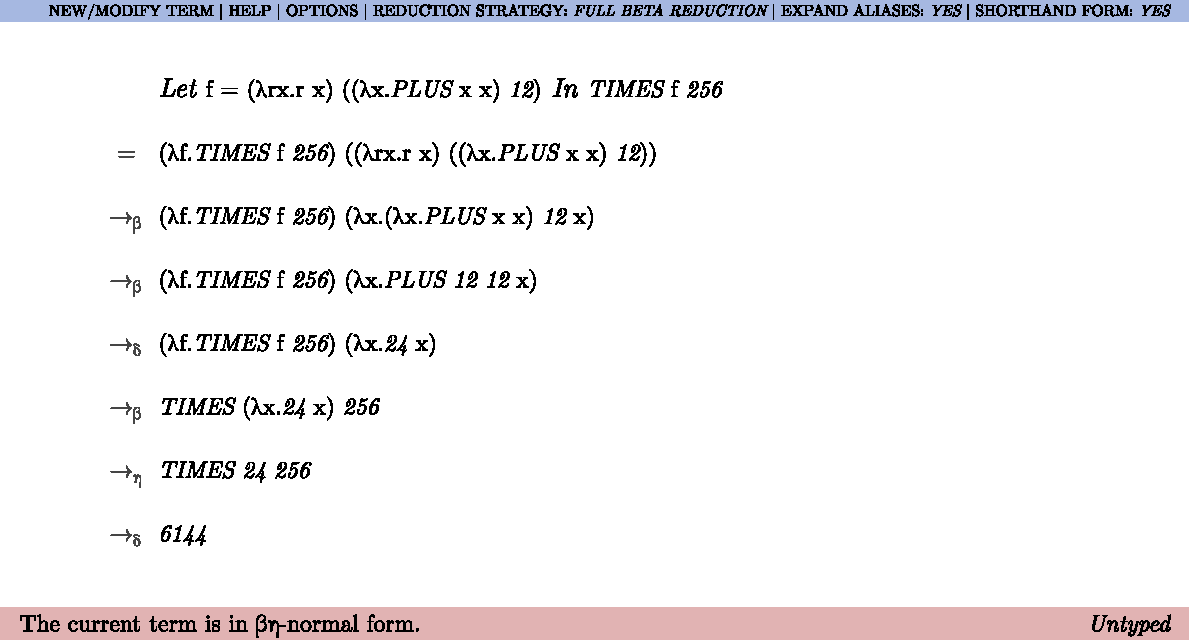
\includegraphics[scale=0.54]{mainscreenprint.pdf}}
\caption{\textit{The main screen. Size of the elements is increased for print.}}\label{mainscrfig}
\end{figure}
\end{center}

\paragraph{Head navigation bar}
On the main screen, the head navigation bar accommodating useful options is always present.
The bar contains an option to return to the initial screen to modify the currently evaluated term,
or enter a new one, a link to the help page, and display and evaluation strategy settings.
Accessible from the \textit{Options} drop-down menu, the alias addition, import and export, and
a conversion to SKI combinators options are available.

\paragraph{Evaluation space}
This area is the essential component of the application, taking up the majority
of the screen estate. The user-input terms are displayed on this surface, with the
evaluation taking place there. The topmost term is the user-input one,
and the terms below are products user-evaluation of the topmost. On the left-hand
side of a term there is an arrow, indicating what kind of redex was used to produce
the term. The evaluation itself is described in Section \ref{sec:eval}.

\paragraph{Bottom panel} The bottom panel is a surface designed to show the information
relevant to the evaluation of a particular term. The information about
a number of each kind of redex present in the term on the last line is displayed,
if a type system is selected, a type of the term or a notification
of a failure to type the term, or when loading from a file,
a number of the loaded terms or aliases. The information is written in a clear and
a complete sentence, communicating the message in a natural manner.
The content of the panel is dependent on the current type system, display settings, and reduction strategy.
As an example, some terms and the corresponding bottom panel messages are given:
\begin{framed}
\hspace{-0.6cm}{\footnotesize
\begin{tabular}{cl}
   $\lambda f.s f$ & The current term is in $\beta$-normal form, and it can be $\eta$-reduced.\\
	$s$ & The current term is in $\beta\eta$-normal form.\\
$(\lambda x.x)\;(\mathit{PLUS}\;\mathit{2}\;\mathit{2})$ & The current term contains 1 beta-redex \textit{\&} 1 delta-redex.\\
$λfgx.f (g x)$ & The current term is in $\beta$-normal form and its type is $\text{\scriptsize$(e \to d) \to (c \to e) \to c \to d$}$.\\
$\lambda a.b$ & The current term has no redexes and it is not typeable.
\end{tabular}
}
\end{framed}

\subsection{User's input}\label{sec:input}
Upon entering the application, the user can immediately begin to type the expression
to be evaluated. The outline of the input box is colored based on the syntactic
correctness of the input term; {\color{synbad}$\blacksquare$} red on syntactically incorrect,
and {\color{syngood}$\blacksquare$} green on
syntactically correct terms, providing a useful and immediate feedback to the user after
each keystroke. As per the information shown on the entry page, in order to
enter the lambda character, the user simply enters the backslash key, which in turn
gets automatically converted into the lambda character, written into the input box.
The type constructor arrow for the simply typed $\lambda$-calculus is input
in a similar fashion, using a succession of a hyphen and a greater-than sign,
the most natural way to write an arrow using a standard keyboard.

To submit a syntactically correct term for an evaluation, a user clicks on the \textit{Submit} button,
or presses the Enter key, entering the \textit{main screen}.

\begin{center}
\begin{figure}[H]\centering
\setlength{\fboxsep}{0pt}%
\setlength{\fboxrule}{0.1pt}
\fbox{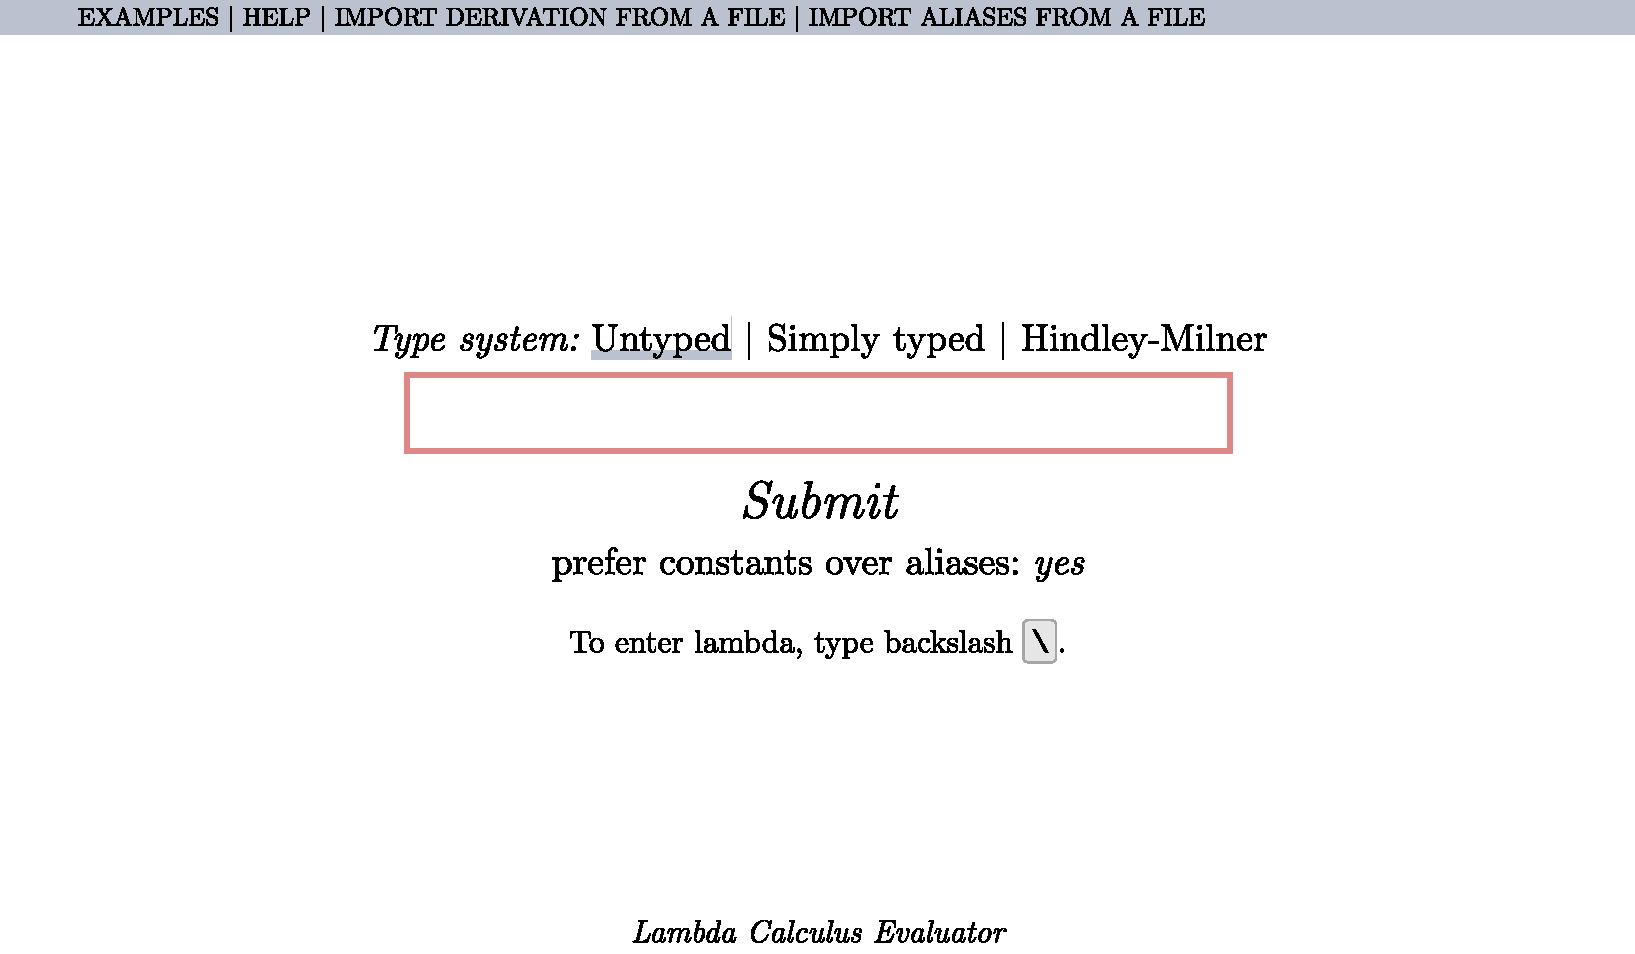
\includegraphics[scale=0.38]{initialScreen.pdf}}
\caption{\textit{The initial screen. Size of the elements is increased for print.}}\label{initscr}
\end{figure}
\end{center}

\noindent

\paragraph{Aliases and constants}
Aliases and constants can be used for input, including Church-encoded numerals up to three digits,
except in the case of employed simply typed $\lambda$-calculus type system which does not
accept Church-encoded data and functions.
An option to disambiguate between conflicting alias- and constant names is available,
delivering interpretation of the names accordingly to the preference set by a user. The default behavior is
to interpret all conflicting names as constants. For instance, the user inputs
a string ``21'': such a string could represent Church-encoded numeral as well as the primitive
value---a constant defined outside the $\lambda$-calculus. Considering the user did not change the default
setting, this string will be parsed as a constant of twenty-one. Occasionally, one may wish
to enter both an alias and a constant. In such case, one can use an exclamation mark
just before the conflicting name to indicate the exception to the preference setting.
Again assuming the default setting, a string ``!FALSE 12 TRUE'' would be interpreted as
$(\lambda xy.y)\;\textit{12}\;\textit{TRUE}$, the constants being written in italic type.

Because of the memory-intensive generation of Church-encoded numerals, a user can input
such numerals only up to three digits. Displaying the terms on the screen is done
by stack-based recursive procedure; rendering large enough numerals, and generally, any terms,
will cause a stack overflow.

\subsection{Evaluation}\label{sec:eval}
After a syntactically valid term has been submitted, one can commence and repeat
the manual, step-by-step evaluation by
mouse-clicking the desired redex inside the expression until a normal form is reached.
The new, reduced expression will be rendered below the clicked one, together
with an arrow indicator of the redex' kind.
As described in Section \ref{sec:red},
under full $\beta$-reduction,
redexes inside the term may be evaluated in an arbitrary order.
If an evaluation strategy other than the full beta-reduction is selected, 
it is possible to select at most one redex, as accorded by the chosen evaluation strategy.
When evaluating untyped terms, the default strategy is full beta-reduction,
otherwise, as formally defined, call by value is used, and the option to change the 
strategy is disabled.
Presence of a redex inside a term is
indicated by an argument- and function color outline, shown on mouse-hover, as illustrated
in Figure \ref{redexfig}. Different kinds of redexes are indicated by an outline of these different colors,
written as hexadecimal triplets, using the RGB color model:
\begin{center}
\begin{tabular}{ll}
	{\color{delta}$\blacksquare$} \texttt{98c6a8}   &$\delta$-redex\\
	{\color{letexpr}$\blacksquare$} \texttt{e6c79b} &$\eta$-redex, \textit{Let} expression\\
	{\color{betaFunc}$\blacksquare$} \texttt{8e8fa7}&$\beta$-redex' function\\
	{\color{betaArg}$\blacksquare$} \texttt{bc8f8f} &$\beta$-redex' argument
\end{tabular}

\vspace{0.3cm}
\rule{7cm}{0.02cm}

\begin{figure}[H]\centering
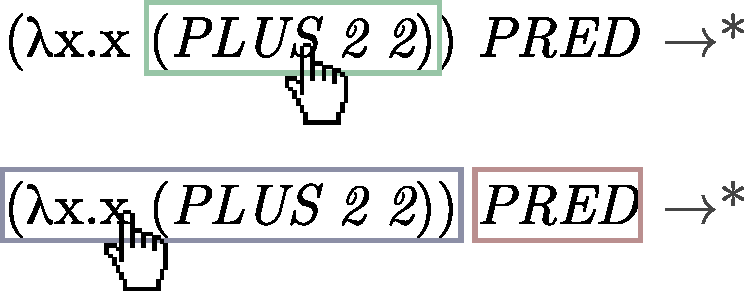
\includegraphics[scale=0.5]{redexes.pdf}
\caption{\textit{A color outline indicating a reducible expression appearing on mouse-hover. The asterisk-arrow
for performing an immediate evaluation is visible following the term.}}\label{redexfig}
\end{figure}
\end{center}
As the user would anticipate, on mouse click, the highlighted expression will be reduced.
The reason behind highlighting the redexes only on mouse-hover, instead of highlighting
them permanently, is twofold: for visual clarity, as a permanent color outline would
create bothersome visual clutter on the screen, and secondly, redexes are
often nested, which would result in confusing outlines bearing no useful information.
In a case of nested redexes, mouse selection is analyzed bottom-up---the deepest 
redex that is pointed at will be chosen. It is not possible to
perform an $\eta$-conversion if some other kind of reduction is available.

\paragraph{Immediate evaluation}
As some of the evaluation chains, or \textit{derivations},
can be rather long, in some cases using
only step-by-step evaluation to reach the normal form would be tiring, or even altogether unfeasible.
To directly evaluate a term at once, one can simply click on an asterisk-arrow following
a reducible term, as visible in Figure \ref{redexfig} towards the right margin.
If a derivation is short enough, precisely, less than 50 evaluation steps,
each evaluation step will be rendered on a new line, as if evaluated manually,
otherwise, only the computed normal form
will be appended to the already rendered derivation, and the information
about the number of taken evaluation steps needed to reach the normal form will be
displayed on the bottom panel. The user-selected reduction strategy 
will be used for an immediate evaluation, except in the case of \textit{full beta-reduction}, where the
\textit{normal order} will be used, as it is complete---if the normal form does
exist, it will eventually be reached.
As the problem of recognizing the non-normalizing terms is generally undecidable,\cit{zlatuska}
the computation may continue indefinitely, without any means
to circumvent or detect such non-terminating computation beforehand.
A simple heuristic terminating execution
of already computed terms in succession is employed.
Eta-redexes are not reduced automatically during the immediate evaluation and they
have to be reduced only manually.

\subsection{Alias management}
Sometimes, it may be useful to assign a name to a commonly used terms. 
Addition of an alias is done via the \textit{Add an alias} dialog box (fig. \ref{aliaswindow}),
accessible from the head navigation bar's \textit{Options}.
The name can be composed of only uppercase alphabetical characters,
and this condition is
reflected in the behavior of the name's input box: firstly, any alphabetical character
will be immediately converted to upper case, and secondly, as non-alphabetical characters
are not admissible for names, it is not possible to enter them into the box at all.

The term to be named is entered in a similar fashion to that of the initial screen;
expectedly, the already defined aliases and constants can be used to define a new alias,
and an already existing name cannot be assigned to another term.
An option to enter the term on the last (\textit{current}) line automatically into the 
input box is available. The color of the input boxes, which are both stylized as line, is changing
based on the syntactic correctness of the input term, or the admissibility of the intended name,
in the same manner as that described in Section~\ref{sec:input} -- User's input.

An alias is assigned only to a particular term; this means that
generally the $\alpha$-equivalent terms do not share the same assigned name,
the name is applied only to a syntactically identical terms.

\begin{figure}[H]\centering
\fbox{
\includegraphics[scale=0.6]{aliaswindow.pdf}}
\caption{\textit{The alias addition dialog box with placeholders describing the expected values.}}\label{aliaswindow}
\end{figure}

\subsection{Display settings}
At any point, it is possible to change the active display setting via the 
head navigation bar options \textit{Expand aliases} and \textit{Shorthand form},
both ranging over binary values. If the alias expansion option is active,
terms will be rendered as the name they carry (fig. \ref{displayopts}). On mouseover, the term will
be shown without the alias expansion, enabling a user to select potentially
aliased or nested reducible expressions. The suitability of the alias expansion is
checked top-to-bottom: would there be a named term $M$ containing another named term $N$,
the name of the term $M$ will be preferred.

The shorthand form option toggles between rendition of terms (and types, if any present)
either as fully parenthesized, or abbreviated,
with unambiguously omitted parentheses, as described in Section \ref{sec:conventions}.

\begin{figure}[H]\centering
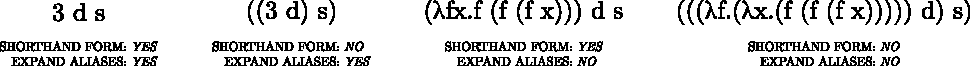
\includegraphics[scale=0.74]{displayopts2.pdf}
\vspace{-0.4cm}
\caption{\textit{A collage of application's term renditions under different settings.}}\label{displayopts}
\end{figure}

\noindent
By default, aliases are expanded, and terms and types are shown in the shorthand form.
Changing any of the two settings will cause an immediate redraw of the terms currently
presented on the screen.

\subsection{Help page}
The \textit{Help} page does serve as a readily available reference, accessible from the 
applications' head navigation bar at all times. Besides the general information about the application
and its use, the help page also contains a number of illustrative $\lambda$-calculus expressions, possible to be
evaluated using the application. To load the mentioned examples to the application, the user simply
selects the term by clicking on it. Additionally, on the help page, one can find
an enumeration of all available predefined aliases and constants.

\subsection{Import and export} \label{sec:io}
At times, one may wish to store an evaluation chain for later retrieval, print the derivation,
or export it as a \LaTeX\;source.
The printing and \LaTeX\;source generation functionality utilizes the active display settings,
namely the alias expansion and shorthand form, thus making the exporting
facility as flexible as the web application's term-displaying abilities themselves.
The import and export options dialog (fig. \ref{iowindow}) is accessible
via the \textit{Options} menu from the head navigation bar.

A quick and convenient way to share or save a term on the current line is to copy the
URL from the web browser's address bar, as the application does encode
the current term in the URL's optional \textit{fragment identifier} part,
initiated with a hash symbol (\texttt{\#}), typically used to point to a particular 
portion of a document.

\begin{figure}[H]\centering
\fbox{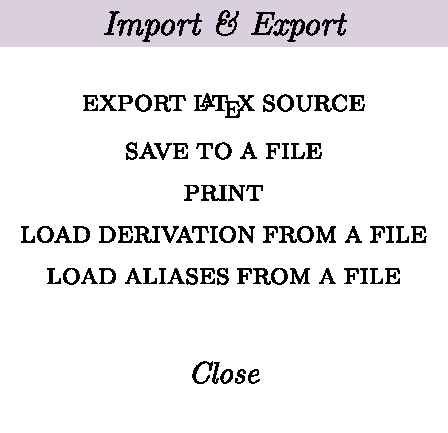
\includegraphics[scale=0.72]{iowindow.pdf}}
\caption{\textit{The ``Import \& Export'' options dialog box.}}\label{iowindow}
\end{figure}

%toto daj na 1 stranu
\paragraph{File input and output}
By user request, a file containing the derivation chain is generated and
downloaded. The default name of the file is \texttt{save.lambda}, and in a human-readable
format, the file holds the information about term on every line, what kind of reduction
did produce the term \textit{(the arrow)}, and the type system used (Figure \ref{fileexample}).
All of the user-defined aliases are also stored inside the file,
as the aliases may be used to display the saved terms, or simply to
enable users to conveniently reuse the already defined aliases in the future;
this is especially useful with a combination of the initial screen feature
allowing loading only the aliases from the file, as these can be used for an input
of a new term right away. When loading a file into the evaluator, the
system prompt looks only for \texttt{*.lambda} files by default.

\begin{figure}[H]
\setlength{\columnsep}{-1cm}
\begin{multicols}{2}
\begin{framed}
\begin{lstlisting}[escapeinside=||]
discipline UNTYPED
alias ADDFIVE (PLUS 5)
term NO ((|\hspace{0.23mm}
\includegraphics[width=0.4em]{lambdachar.pdf}\hspace{0.23mm}|x1.((PLUS 5) x1)) 4)
term BETA ((PLUS 5) 4)
term DELTA 9
\end{lstlisting}
\end{framed}
\columnbreak
\begin{align*}
\quad\quad&(\lambda x_{1}.\mathrm{ADDFIVE}\;x_{1})\;\mathit{4}\\
\quad\quad\to_\beta\quad&\mathrm{ADDFIVE}\;\mathit{4}\\
\quad\quad\to_\delta\quad&\mathit{9}
\end{align*}
\end{multicols}
\vspace{-0.5cm}
\caption{\textit{Human-readable file text (left) and the corresponding resulting
derivation after a loading (right).
The \LaTeX\;source code of the resulting derivation is shown in fig. \ref{latexexample}.}}\label{fileexample}
\end{figure}

\noindent
The $\mathit{File}$ adheres to an intelligible structure, where
each line is initiated with a keyword specifying the content of the line,
followed by the actual data.
In the resulting derivation, the terms are ordered the same way they appear in the file,
otherwise, an order of the elements is not relevant.
Formally, the syntax of the file is given by the following grammar, where the $\mathit{Name}$,
as defined previously, is a string of uppercase letters, with terminals written
using a monospaced typeface, where \texttt{\textbackslash n} represents the newline character:

\vspace{3mm}
\begin{tabular}{rlll}
$\mathit{Line}$ &$::=$ &\texttt{alias}\;\;$\mathit{Name}\;\;M$ & \\
    &\hspace{0.1cm}$|$ &\texttt{term}\;\;$\mathit{Arrow}\;\;M$  & \\
    &\hspace{0.1cm}$|$ &\texttt{discipline}\;\;$\mathit{TypeSystem}$ & \\
$\mathit{Arrow}$ &$::=$             &\texttt{NO}\;\;$|$\;\;\texttt{BETA}\;\;$|$\;\;\texttt{ETA}\;\;$|$\;\;\texttt{DELTA}\;\;$|$\;\;\texttt{EQ}  &\\
$\mathit{TypeSystem}$ &$::=$   &\texttt{UNTYPED}\;\;$|$\;\;\texttt{HINDLEY\_MILNER}\;\;$|$\;\;\texttt{SIMPLY\_TYPED}&\\
$\mathit{File}$ &$::=$             &$\varepsilon\;\;|\;\;\mathit{Line}$\texttt{\textbackslash n}$\mathit{File}$&
\end{tabular}

\paragraph{\LaTeX\;source code generation}
The exported evaluation chain is typeset using the \texttt{align*} environment,
available through the popular \texttt{amsmath} package, which is required for
any \LaTeX\;distribution\footnote{\url{https://ctan.org/pkg/required/}}---the
user has to include the \verb|\usepackage{amsmath}| declaration in the 
preamble of their document. On export, a new browser window
will be opened, containing the \LaTeX\; source code of the derivation as plain text.
Before exporting a derivation, one should make sure that the desired
displaying options are in place, as these will be used to generate the code to
make the compiled result look essentially the same as the derivation shown on the application screen.
In the same manner as on the  
application screen, constants are set in italic type, and aliases are set in roman type.

\begin{figure}[H]
\begin{framed}
\begin{verbatim}
% don't forget to \usepackage{amsmath}
\begin{align*}
&(\lambda x_{1}.\mathrm{ADDFIVE}\;x_{1})\;\mathit{4}\\
\to_\beta\quad&\mathrm{ADDFIVE}\;\mathit{4}\\
\to_\delta\quad&\mathit{9}
\end{align*}
\end{verbatim}
\vspace{-0.3cm}
\end{framed}
\vspace{-0.4cm}
\caption{\textit{An example of a generated \LaTeX\;code, setting the derivation shown
in fig. \ref{fileexample}.}}\label{latexexample}
\end{figure}

\paragraph{Printing} Derivation printing is realized via the usual system-provided prompt,
using a customized style sheet, describing a page layout for the printing. Notable changes,
compared to the application's screen, are hiding the user interface elements, particularly
head navigation bar and the bottom panel, modifying text overflow and page margin settings, and
decoloring visible elements, e.g. the background, which has a slightly grey tint.
The system printing dialog can be invoked via the \textit{Import \& Export} window,
or using the web browser interface, and it is commonly accessible via the keyboard shortcut \texttt{ctrl + p}.

\section{Comparison with existing solutions}
There are several existing applications for evaluating lambda calculus expressions available online.
In order to justify the existence of yet another,
a qualitative comparison of multiple features of six of the existing solutions to this work's is given in the
following table:

\begin{table}[H]
\centering
\label{comparisonTable}
\resizebox{\textwidth}{!}{%
\begin{tabular}{|c||c|c|c|c|c|c|}
\hline
\textbf{} & \textbf{aliases} & \textbf{reduction strategies} & \textbf{\begin{tabular}[c]{@{}c@{}}step-by-step\\ evaluation\end{tabular}} & \textbf{import \& export} & \textbf{type systems} & \textbf{lambda input} \\ \hhline{|=#=|=|=|=|=|=|}
\textit{\textbf{this work}} & \cellcolor[HTML]{BFE1C0}\begin{tabular}[c]{@{}c@{}}yes,\\ input and output,\\programmatic Church numerals\end{tabular} & \cellcolor[HTML]{BFE1C0}\begin{tabular}[c]{@{}c@{}}normal order,\\ applicative order,\\ call by value,\\ call by name\end{tabular} & \cellcolor[HTML]{BFE1C0}yes & \cellcolor[HTML]{BFE1C0}\begin{tabular}[c]{@{}c@{}}file,\\ URL,\\ \LaTeX\end{tabular} & \cellcolor[HTML]{BFE1C0}\begin{tabular}[c]{@{}c@{}}simply typed\\ $\lambda$-calculus,\\ Hindley-Milner\\ type system\end{tabular} & \textbackslash\;\;\textit{and} λ \\ \hhline{|=#=|=|=|=|=|=|}
\cite{Interpreter1} & \cellcolor[HTML]{DBB8B8}no & \cellcolor[HTML]{DBB8B8}normal order & \cellcolor[HTML]{DBB8B8}\begin{tabular}[c]{@{}c@{}}no,\\ displays\\ intermediate\\ results\end{tabular} & \cellcolor[HTML]{DBB8B8}\begin{tabular}[c]{@{}c@{}}no options\\ available\end{tabular} & \cellcolor[HTML]{DBB8B8}\begin{tabular}[c]{@{}c@{}}no options\\ available\end{tabular} & lambda \\ \hline
\cite{Interpreter2} & \cellcolor[HTML]{DBB8B8}no & \cellcolor[HTML]{DBB8B8}call by value & \cellcolor[HTML]{DBB8B8}no & \cellcolor[HTML]{DBB8B8}\begin{tabular}[c]{@{}c@{}}no options\\ available\end{tabular} & \cellcolor[HTML]{DBB8B8}\begin{tabular}[c]{@{}c@{}}no options\\ available\end{tabular} & \textasciicircum  \\ \hline
\cite{Interpreter3} & \cellcolor[HTML]{BFE1C0}\begin{tabular}[c]{@{}c@{}}yes,\\ input and output\end{tabular} & \cellcolor[HTML]{BFE1C0}\begin{tabular}[c]{@{}c@{}}lazy evaluation,\\ eager evaluation,\\ normal order\end{tabular} & \cellcolor[HTML]{DBB8B8}\begin{tabular}[c]{@{}c@{}}no,\\ displays\\ intermediate\\ results\end{tabular} & \cellcolor[HTML]{BFE1C0}\begin{tabular}[c]{@{}c@{}}option to export\\ user-defined aliases\end{tabular} & \cellcolor[HTML]{DBB8B8}\begin{tabular}[c]{@{}c@{}}no options\\ available\end{tabular} & \textbackslash \\ \hline
\cite{Interpreter4} & \cellcolor[HTML]{BFE1C0}yes, input only & \cellcolor[HTML]{DBB8B8}\textit{not listed} & \cellcolor[HTML]{DBB8B8}no & \cellcolor[HTML]{DBB8B8}\begin{tabular}[c]{@{}c@{}}no options\\ available\end{tabular} & \cellcolor[HTML]{DBB8B8}\begin{tabular}[c]{@{}c@{}}no options\\ available\end{tabular} & \textbackslash\;\;\textit{and} λ \\ \hline
\cite{Interpreter5} & \cellcolor[HTML]{BFE1C0}\begin{tabular}[c]{@{}c@{}}yes,\\ via let expressions,\\ input only\end{tabular} & \cellcolor[HTML]{DBB8B8}\textit{not listed} & \cellcolor[HTML]{DBB8B8}no & \cellcolor[HTML]{DBB8B8}\begin{tabular}[c]{@{}c@{}}no options\\ available\end{tabular} & \cellcolor[HTML]{DBB8B8}\begin{tabular}[c]{@{}c@{}}no options\\ availabe\end{tabular} & \textbackslash \\ \hline
\cite{Interpreter6} & \cellcolor[HTML]{BFE1C0}\begin{tabular}[c]{@{}c@{}}yes,\\ input and output\end{tabular} & \cellcolor[HTML]{BFE1C0}\begin{tabular}[c]{@{}c@{}}normal order,\\ call by name,\\ head spine reduction,\\ call by value,\\ applicative order,\\ hybrid normal order,\\ hybrid applicative order\end{tabular} & \cellcolor[HTML]{BFE1C0}yes & \cellcolor[HTML]{DBB8B8}\begin{tabular}[c]{@{}c@{}}no options\\ available\end{tabular} & \cellcolor[HTML]{DBB8B8}\begin{tabular}[c]{@{}c@{}}no options\\ available\end{tabular} & \textbackslash \\ \hline
\end{tabular}%
}
\caption{\textit{A comparison with existing web $\lambda$-calculus evaluators.}}
\end{table}

\noindent
Besides often missing useful features and an ease of use,
some of the applications were unable to carry out even the more basic tasks,
for instance accepting shorthand input, evaluating inputs of a still reasonably large size,
or lacking the desired input-output idempotence.

\newpage
\chapter{Implementation}
Using the three core web development technologies,
HTML \textit{(Hypertext Markup Language)}, CSS \textit{(Cascading Style Sheets)}, and JavaScript,
the evaluator is built as a single-page application,
i.e. an application using solely dynamic modifications of the content of the current page,
as opposed to redirecting, reloading, or downloading a page with a new content.
Using a web browser as an application platform contributes
to the application's compatibility and availability, 
as there is no need for an installation on the target system.
The application is static---it is executed exclusively on the client-side,
in case of an actual deployment alleviating the server load on one hand,
allowing for downloading and subsequent offline usage by a user on the other.
The application has no external dependencies in terms of frameworks, libraries, or
fonts, and is entirely self-contained.

The application is written using a modern JavaScript standard---the 6\textsuperscript{th} edition of ECMAScript,
providing many useful features, for instance the new syntax for object definition (``classes''), or
lambda expressions (``arrow functions'').\footnote{\url{http://es6-features.org/}}
Would the JavaScript be disabled in the user's browser, an appropriate notification will be displayed.

To tightly control the application's typography across many different systems,
the \textit{Computer Modern} typeface, licensed under a free and open-source SIL
Open Font License,\footnote{\url{http://scripts.sil.org/OFL/}.}
is distributed along the application, allowing
for consistent user experience and arguably {\ae}sthetically pleasing visual appearance of the application.

The authorial source code is licensed under a public
domain CC0 license,\footnote{\url{https://creativecommons.org/publicdomain/zero/1.0/}}
allowing anybody to reuse and improve the work for any purpose and with no restrictions whatsoever.

\section{Operation}
The application works by programmatically modifying
elements of the \textit{Document Object Model} (DOM)---a tree
structure with nodes representing parts of a document---based
on the user's actions and the application's state. The application's evaluation
operates in a working cycle initiated by a user action:
first, after the user action has
occurred (e.g. clicking on a textually represented redex), the application
identifies and fetches the corresponding internal term-representation object,
then, using the logic system's rules, a new term is produced and the
internal representation is updated, and finally, the changes are reflected
on the external (screen) representation of the derivation chain.

\paragraph{HTML structure and DOM}
Both of the application's screens are described in a single hypertext markup \texttt{index.html} file (fig. \ref{html}).
By programmatic modification of the tree structure,
these screens, and also the dialog windows, are being
displayed or hidden using the setting of an appropriate CSS attributes to
the nodes. The presentation of the currently evaluated terms is realized
by inserting a procedurally generated HTML code into
the designated node, \texttt{evaluationFrame}, using the \texttt{Element.innerHTML} utility provided by the
DOM API.\footnote{\url{https://developer.mozilla.org/en-US/docs/Web/API/Element/innerHTML/}}

\begin{figure}[H]\centering
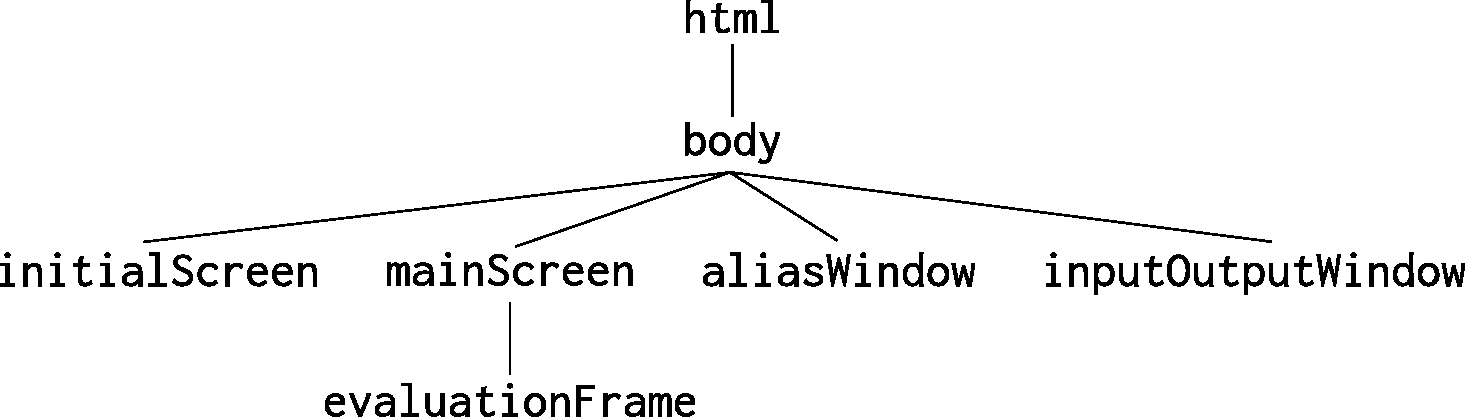
\includegraphics[scale=0.35]{htmlstructure.pdf}
\caption{\textit{An abridged structure of the application's HTML markup.}}\label{html}
\end{figure}

\paragraph{Text input processing}
A top-down recursive descent parser, implemented using a single \texttt{Parser} object,
is used to translate the user's input text into an
internal data structure: for each of the production rules of the grammar there exists
a procedure deciding whether the currently parsed text is generated by the respective production rule.
The expected input is short (dozens of characters), which allows use of an implementation with an arbitrary
look-ahead, straightforwardly applying trial-and-error method for each of the rules,
trading off efficiency for simplicity.\cit{compilers} To enable a use of
the shorthand notation, a preprocessor, working on a textual level, is
employed to fill in the missing parentheses, bypassing problems connected
with parsing the shorthand form's left-recursive grammar.

\paragraph{Mouse redex highlighting processing}
As it is described in Section \ref{sec:eval}, mouse-hover events on terms on the screen
invoke a color outline around a deepest pointed-at reducible expression, as
portrayed in Figure \ref{redexfig}. Although visual
change on mouse-hover event is natively supported by CSS,
in this context, using only the CSS would not be sufficient, as
reducible expressions can be nested, which would
instigate coloring not only of a one reducible expression, but also
of all its parent elements---this problem is solved
programmatically using JavaScript. When a HTML code of a term is 
generated, \texttt{class} markers are used to indicate a reducible expression
inside a term,
invisible at the time. On mouse-hover event, a function is called with
the pointed-at DOM object passed as an argument. If the object is marked
as a redex, the function swaps the \texttt{class} marker for another,
triggering a CSS outline appearance, and terminating, otherwise, it is called for the parent element
until it succeeds, or it is being applied outside of a reasonable scope.

\paragraph{Mouse redex clicking processing}
A mouse click processing is a bit more involved, as the particular
term on screen, which has been clicked on, has to be identified
within the internal representation,
in order to be evaluated, for a term can contain multiple redexes. This identification is achieved by
making each terminal symbol a button during the HTML generation,
signalling what term is being clicked on, using a simple binary tree
prefix encoding, where an empty string does denote the root of a tree,
and \texttt{0} and \texttt{1} do denote the left, respectively the right subtree (fig. \ref{encoding}).
A part of the term interface, the \texttt{fromCode} method is used
to fetch the requested subterm within the internal representation, optionally
returning the pointed-at redex instead of the exact subterm.

The encoding of a term's position within the derivation chain is straightforward;
the code of a term is prefixed with a line number (indexed by zero), followed by a point character (dot). For instance,
the code \texttt{2.1} would represent the right subtree of a term on the third line
of the derivation chain.

\begin{figure}[H]\centering
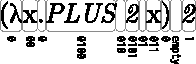
\includegraphics[scale=1.63]{encoding.pdf}
\caption{\textit{An example of a subterm encoding, enabling an identification of the clicked term.}}\label{encoding}
\end{figure}

\paragraph{Evaluation}
The evaluation itself is realized via the \texttt{Evaluator} object, which contains a library of
static\footnote{Static method is a member function not bound to a specific instance, but rather the whole class. Because
the \texttt{Evaluator} is a single object that is not an instance of any class, these methods are, in fact, bound to it's instance, thus are not
static in a conventional sense.} methods designated to term evaluation and manipulation,
containing redex identification, redex fetching, optionally taking into consideration
the evaluation strategy or a particular redex kind, for
instance \texttt{Evaluator.getRedex.eta}, or more general-purpose
functions, such as \texttt{Evaluator.isValue}, or the ubiquitous \texttt{Evaluator.substitute}.

The \texttt{Evaluator} employs the static methods of the \texttt{Type} class when dealing
with typed terms, and utilizes the application's
state---for example the current type system settings---by accessing
the main object's \texttt{OLCE.Settings} properties.

\section{Structure}
Object-oriented programming paradigm, supported by JavaScript, is employed
to model the data, as \textit{objects} can closely match the term structure,
e.g. a \textit{term} can be represented by an interface, an \textit{abstraction} can
be an implementation thereof, closely matching the lambda calculus' grammar.
Due to the JavaScript's dynamic nature, the mentioned interface is only implicit,
as there is no syntactic support for such a construct in the language itself.
Moreover, the language lacks a conventional \textit{class} semantics, and
it is rather centered around \textit{objects}. The \texttt{class} syntax,
present in newer standards of JavaScript, is
an syntactic sugar over the language's existing prototype-based
inheritance model.\footnote{\url{https://developer.mozilla.org/en-US/docs/Web/JavaScript/Reference/Classes}}

The names of source code files do approximately match the object definitions they contain,
and are briefly described in the Appendix \ref{dix:files}.

\begin{figure}[H]\centering
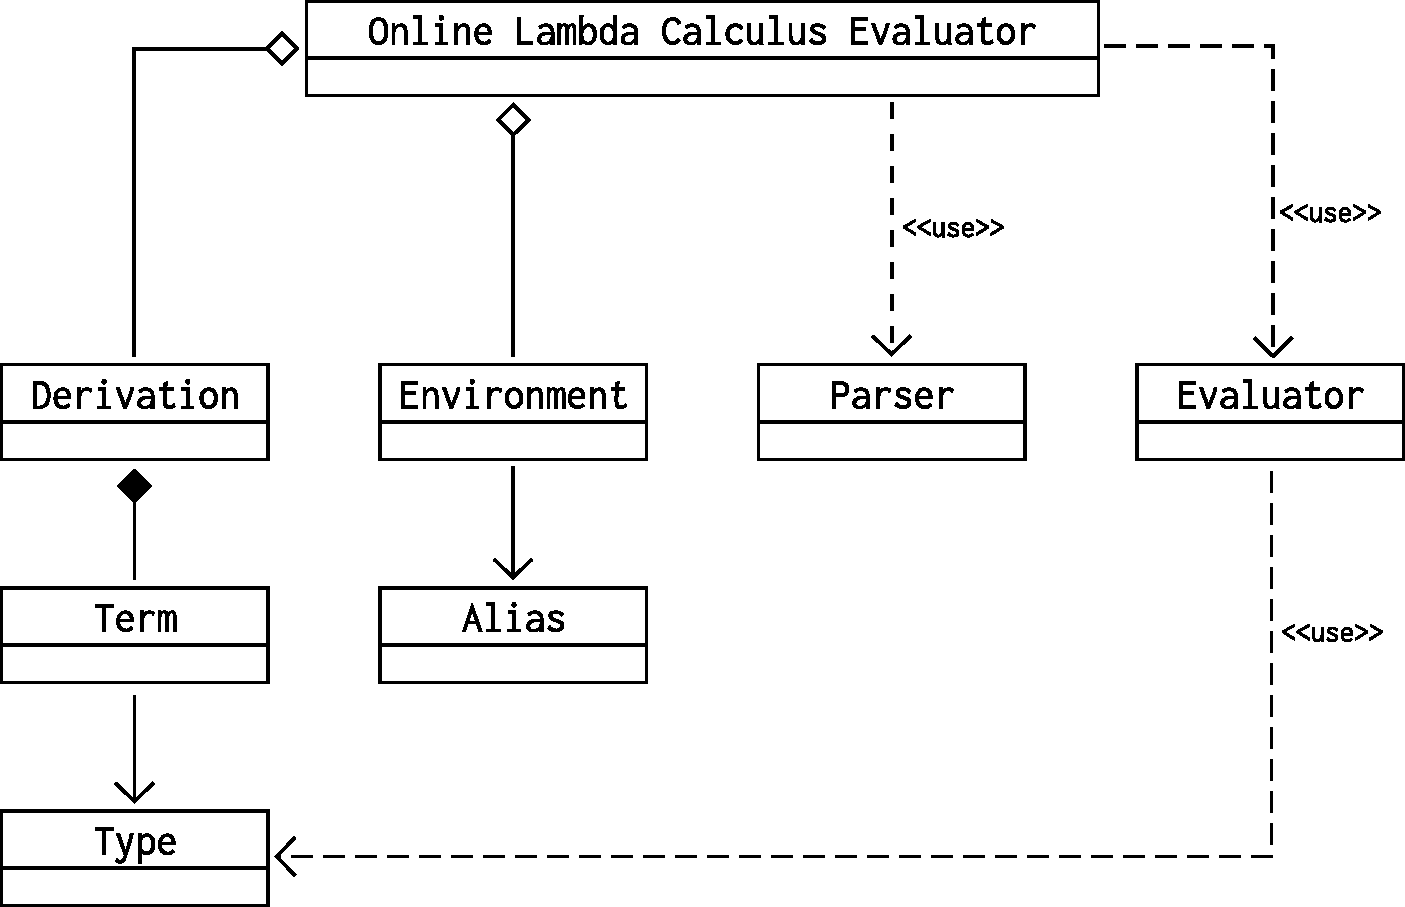
\includegraphics[scale=0.33]{simpleUMLpdf.pdf}
\caption{\textit{A simplified class diagram of the project.}}\label{uml}
\end{figure}

\paragraph{The entry point}
The application itself is structured as a single object (named \texttt{OLCE}), containing
a number of methods for direct DOM manipulation, and methods which are
triggered by a user action---mouse or keyboard events.
Generally, every control element of the application, e.g. a button, does have a corresponding
\texttt{OLCE.UI} method, which gets invoked on the element's interaction, for instance on a button click.
The data members of the \texttt{OLCE} object include a collection of the application's
settings (e.g. how to display terms), DOM object references (e.g. where to render and display terms),
the user- and predefined aliases, and the currently evaluated
derivation chain (what terms to display). On a page load, the \texttt{OLCE.DOM.prepare()} associates
the page elements with references for a rapid and a systematic further access by methods.

\paragraph{Internal representation}
The evaluated terms, as presented on the screen, are contained in
the \texttt{Derivation} class, which is a singly linked list,
extended with a functionality to generate a HTML code of the derivation chain,
a \LaTeX\; code, or to generate a file text for a subsequent downloading.
Each instance of the \texttt{Derivation}---each node of the list---does contain
a single \texttt{Term} object, and a kind of reduction that produced the term (i.e. an arrow).

\begin{figure}[H]\centering
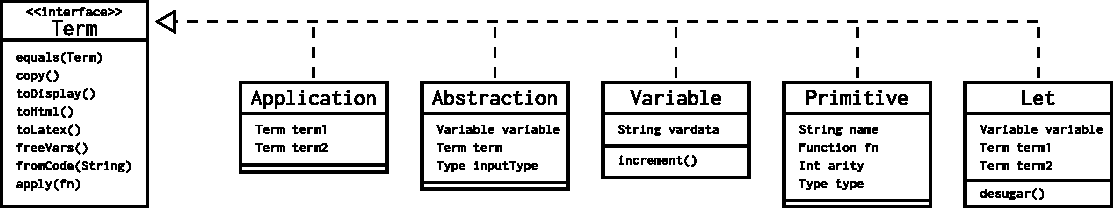
\includegraphics[scale=0.64]{termUML.pdf}
\caption{\textit{Object term representation using an implicit interface.}}\label{termuml}
\end{figure}

\noindent
Because JavaScript is a dynamically typed language, a suitability of an object
for a method call
is determined by a presence of the method in the object, rather than by a type of the object.
For this, the subtype polymorphism is no longer needed, the object just needs to be 
checked for an implementation of a desired call---consequently, the language
lacks an explicit interface support present in more conventional,
statically typed object-oriented programming languages, such as
Java, or C++ (as abstract classes). For a better understanding, this interface is imagined, as to
express the need for an implementation of particular methods by some other
application component.

As can be seen in Figure \ref{termuml}, the object structure is closely matching the logic system's
syntactical structure (cf. Section \ref{sec:hm}'s term grammar)---an abstraction enabling
a clear reflection upon the internals of the evaluator system.

\section{Compatibility and performance}
The application is intended for use on personal computers equipped with a mouse
or a trackpad, for it relies on mouse events, such as mouse-over for redex highlighting,
and due to this fact, an experience on devices with smaller
screens, such as tablets or smartphones,
may be impractical and less satisfactory, although technically attainable.

The support of ES6 features is in modern web browsers practically complete,\footnote{\url{https://kangax.github.io/compat-table/es6/}}
and the application
does not use any non-standard features or APIs,
resulting in a product that is compatible with a wide range of target systems.
The apparently only possibly occurring, cosmetic issues seem to be connected to
support for the CSS' \texttt{box-shadow} property in older Microsoft and Apple browsers,
which are nowadays seldom used.

A large section of the application's functionality is based on recursive procedures,
as these are closely resembling the logic system's rules (for instance,
the inductive definition of the substitution presented in Section \ref{sec:subst}),
which are prone to stack overflow issues on very large inputs. Furthermore,
due to the extensive feature set of the application---for
example counting all the reducible expressions within a term in order
to display such an information---the evaluator
does carry out a numerous computational tasks on each step of the evaluation,
which may be, in some cases, slowing-down the application.
A decision to trade off some efficiency and ``premature optimizations'' for code
simplicity and readability has been made.

\newpage
\chapter{Conclusion}
A lambda calculus evaluator application has been designed and implemented,
providing rich feature set containing an optional step-by-step evaluation,
multiple reduction strategies to choose from, term aliasing support with numerous predefined such aliases,
besides the untyped system, \textit{simple} and Hindley-Milner type system,
various import and export options, including printing, flexible \LaTeX\;source code generation,
URL link generation, file input and output, a convenient help page,
and several display preferences---an application that could hopefully be considered user-friendly
and visually engaging,
and it is, indeed, online.

Possible enhancements of the application would include some code optimizations, an implementation
of automatically $\alpha$-convertible aliases, that could be especially useful 
when dealing with Church encoding, with necessary variable renaming occurring in the course of an
evaluation, an addition of a support for lists and tuples along with an appropriate syntactic sugar,
enabling users to enjoy the infix notation,
or perhaps an implementation of Girard's System F.

\appendix
\chapter{Predefined constants and aliases}\label{app:con}
\vspace{1cm}
%%%%%%%%%%%%%%%%%%%%%%%%%%%%%%%%%%%%%%%%%%%%%%%%%%%%%%%%%%%%%%%%%%%%%%%%%%%%%%%%%%%%%%%%%%%%%%%%%%%%
\begin{table}[H]\scriptsize
\centering
\label{enumeration}
\begin{tabular}{cclcl}
\hline
\multicolumn{1}{|l|}{}                        & \multicolumn{2}{c|}{\Large Alias}                                                                                                           & \multicolumn{2}{c|}{\Large Constant}                                                                                                                                                                        \\ \hline
\multicolumn{1}{|c|}{\textit{name}}           & \multicolumn{2}{c|}{\textit{description and term}}                                                                                          & \multicolumn{1}{c|}{\textit{arity}}     & \multicolumn{1}{c|}{\textit{description}}                                                                                                                         \\ \hhline{|=|=|=|=|=|}
\multicolumn{1}{|c|}{\multirow{2}{*}{$n$}}    & \multicolumn{2}{l|}{\begin{tabular}[c]{@{}l@{}}Church encoded natural numbers $n \in \mathbb{N}$,\\ input up to 3 digits only\end{tabular}} & \multicolumn{1}{c|}{\multirow{2}{*}{0}} & \multicolumn{1}{l|}{\multirow{2}{*}{\begin{tabular}[c]{@{}l@{}}integer $n \in \mathbb{Z}$ primitives. JavaScript\\ implementation-defined range\end{tabular}}}    \\ \cline{2-3}
\multicolumn{1}{|c|}{}                        & \multicolumn{2}{c|}{$\text{\tiny$\lambda f.\lambda x.f^n x$}$}                                                                              & \multicolumn{1}{c|}{}                   & \multicolumn{1}{l|}{}                                                                                                                                             \\ \hline
\multicolumn{1}{|c|}{\multirow{2}{*}{SUCC}}   & \multicolumn{2}{l|}{successor function on Chuch numerals}                                                                                   & \multicolumn{1}{c|}{\multirow{2}{*}{1}} & \multicolumn{1}{l|}{\multirow{2}{*}{successor function on constants}}                                                                                             \\ \cline{2-3}
\multicolumn{1}{|c|}{}                        & \multicolumn{2}{c|}{$\lambda nfx.f\;(n\;f\;x)$}                                                                                             & \multicolumn{1}{c|}{}                   & \multicolumn{1}{l|}{}                                                                                                                                             \\ \hline
\multicolumn{1}{|c|}{\multirow{2}{*}{PRED}}   & \multicolumn{2}{l|}{predecessor function, the least result is zero}                                                                         & \multicolumn{1}{c|}{\multirow{2}{*}{1}} & \multicolumn{1}{l|}{\multirow{2}{*}{\begin{tabular}[c]{@{}l@{}}predecessor function,\\ negative results allowed\end{tabular}}}                                    \\ \cline{2-3}
\multicolumn{1}{|c|}{}                        & \multicolumn{2}{c|}{$\lambda nfx.n\;(\lambda gh.h\;(g\;f))\;(\lambda u.x)\;(\lambda u.u)$}                                                  & \multicolumn{1}{c|}{}                   & \multicolumn{1}{l|}{}                                                                                                                                             \\ \hline
\multicolumn{1}{|c|}{\multirow{2}{*}{PLUS}}   & \multicolumn{2}{l|}{addition function on Church numerals}                                                                                   & \multicolumn{1}{c|}{\multirow{2}{*}{2}} & \multicolumn{1}{l|}{\multirow{2}{*}{addition function on constants}}                                                                                              \\ \cline{2-3}
\multicolumn{1}{|c|}{}                        & \multicolumn{2}{c|}{$\lambda mnfx.m\;f\;(n\;f\;x)$}                                                                                         & \multicolumn{1}{c|}{}                   & \multicolumn{1}{l|}{}                                                                                                                                             \\ \hline
\multicolumn{1}{|c|}{\multirow{2}{*}{MINUS}}  & \multicolumn{2}{l|}{substraction on Church numerals, the least result is zero}                                                              & \multicolumn{1}{c|}{\multirow{2}{*}{2}} & \multicolumn{1}{l|}{\multirow{2}{*}{\begin{tabular}[c]{@{}l@{}}substraction on constants,\\ negative results allowed\end{tabular}}}                               \\ \cline{2-3}
\multicolumn{1}{|c|}{}                        & \multicolumn{2}{c|}{$\lambda mn. n\;\mathrm{PRED}\;m$}                                                                                      & \multicolumn{1}{c|}{}                   & \multicolumn{1}{l|}{}                                                                                                                                             \\ \hline
\multicolumn{1}{|c|}{\multirow{2}{*}{TIMES}}  & \multicolumn{2}{l|}{multiplication on Church numerals}                                                                                      & \multicolumn{1}{c|}{\multirow{2}{*}{2}} & \multicolumn{1}{l|}{\multirow{2}{*}{multiplication function on constants}}                                                                                        \\ \cline{2-3}
\multicolumn{1}{|c|}{}                        & \multicolumn{2}{c|}{$\lambda mnf.m\;(n\;f)$}                                                                                                & \multicolumn{1}{c|}{}                   & \multicolumn{1}{l|}{}                                                                                                                                             \\ \hline
\multicolumn{1}{|c|}{\multirow{2}{*}{ISZERO}} & \multicolumn{2}{l|}{\begin{tabular}[c]{@{}l@{}}predicate testing if a Church numeral is zero,\\ returning Church Boolean\end{tabular}}      & \multicolumn{1}{c|}{\multirow{2}{*}{1}} & \multicolumn{1}{l|}{\multirow{2}{*}{\begin{tabular}[c]{@{}l@{}}predicate testing is a numeral constant\\ is zero\end{tabular}}}                                   \\ \cline{2-3}
\multicolumn{1}{|c|}{}                        & \multicolumn{2}{c|}{$\lambda n.n\;(\lambda x.\mathrm{FALSE})\;\mathrm{TRUE}$}                                                               & \multicolumn{1}{c|}{}                   & \multicolumn{1}{l|}{}                                                                                                                                             \\ \hline
\multicolumn{1}{|c|}{\multirow{2}{*}{LEQ}}    & \multicolumn{2}{l|}{\begin{tabular}[c]{@{}l@{}}predicate testing if a Church numeral is less than,\\ or equal to another\end{tabular}}      & \multicolumn{1}{c|}{\multirow{2}{*}{2}} & \multicolumn{1}{l|}{\multirow{2}{*}{\begin{tabular}[c]{@{}l@{}}predicate testing if a numeral constant\\ is less than, or equal to another\end{tabular}}}         \\ \cline{2-3}
\multicolumn{1}{|c|}{}                        & \multicolumn{2}{c|}{$\lambda mn.\mathrm{ISZERO}\;(\mathrm{MINUS}\;m\;n)$}                                                                   & \multicolumn{1}{c|}{}                   & \multicolumn{1}{l|}{}                                                                                                                                             \\ \hline
\multicolumn{1}{|c|}{\multirow{2}{*}{DIV}}    & \multicolumn{2}{l|}{division on Church numerals}                                                                                            & \multicolumn{1}{c|}{\multirow{2}{*}{2}} & \multicolumn{1}{l|}{\multirow{2}{*}{division function on integer constants}}                                                                                      \\ \cline{2-3}
\multicolumn{1}{|c|}{}                        & \multicolumn{2}{l|}{\textit{recursive definition below}}                                                                                    & \multicolumn{1}{c|}{}                   & \multicolumn{1}{l|}{}                                                                                                                                             \\ \hline
\multicolumn{1}{|c|}{\multirow{2}{*}{EQ}}     & \multicolumn{2}{l|}{predicate testing if two Church numerals are equal}                                                                     & \multicolumn{1}{c|}{\multirow{2}{*}{2}} & \multicolumn{1}{l|}{\multirow{2}{*}{\begin{tabular}[c]{@{}l@{}}equality function on numerical constants,\\ returns Boolean constant\end{tabular}}}                \\ \cline{2-3}
\multicolumn{1}{|c|}{}                        & \multicolumn{2}{c|}{$\lambda mn.\mathrm{AND}\;(\mathrm{LEQ}\;m\;n)\;(\mathrm{LEQ}\;n\;m)$}                                                  & \multicolumn{1}{c|}{}                   & \multicolumn{1}{l|}{}                                                                                                                                             \\ \hline
\multicolumn{1}{|c|}{\multirow{2}{*}{TRUE}}   & \multicolumn{2}{l|}{Church Boolean true}                                                                                                    & \multicolumn{1}{c|}{\multirow{2}{*}{0}} & \multicolumn{1}{l|}{\multirow{2}{*}{Boolean true constant}}                                                                                                       \\ \cline{2-3}
\multicolumn{1}{|c|}{}                        & \multicolumn{2}{c|}{$\lambda xy.x$}                                                                                                         & \multicolumn{1}{c|}{}                   & \multicolumn{1}{l|}{}                                                                                                                                             \\ \hline
\multicolumn{1}{|c|}{\multirow{2}{*}{FALSE}}  & \multicolumn{2}{l|}{Church Boolean false}                                                                                                   & \multicolumn{1}{c|}{\multirow{2}{*}{0}} & \multicolumn{1}{l|}{\multirow{2}{*}{Boolean false constant}}                                                                                                      \\ \cline{2-3}
\multicolumn{1}{|c|}{}                        & \multicolumn{2}{c|}{$\lambda xy.y$}                                                                                                         & \multicolumn{1}{c|}{}                   & \multicolumn{1}{l|}{}                                                                                                                                             \\ \hline
\multicolumn{1}{|c|}{\multirow{2}{*}{ITE}}    & \multicolumn{2}{l|}{conditional, the first argument is Church Boolean}                                                                      & \multicolumn{1}{c|}{\multirow{2}{*}{3}} & \multicolumn{1}{l|}{\multirow{2}{*}{\begin{tabular}[c]{@{}l@{}}conditional, the first argument Boolean constant,\\ type system dependent semantics\end{tabular}}} \\ \cline{2-3}
\multicolumn{1}{|c|}{}                        & \multicolumn{2}{c|}{$\lambda xyz.x\;y\;z$}                                                                                                  & \multicolumn{1}{c|}{}                   & \multicolumn{1}{l|}{}                                                                                                                                             \\ \hline
\multicolumn{1}{|c|}{\multirow{2}{*}{OR}}     & \multicolumn{2}{l|}{logical conjunction on Church Booleans}                                                                                 & \multicolumn{1}{c|}{\multirow{2}{*}{2}} & \multicolumn{1}{l|}{\multirow{2}{*}{logical conjunction on Boolean constants}}                                                                                    \\ \cline{2-3}
\multicolumn{1}{|c|}{}                        & \multicolumn{2}{c|}{$\lambda yx.y\;y\;x$}                                                                                                   & \multicolumn{1}{c|}{}                   & \multicolumn{1}{l|}{}                                                                                                                                             \\ \hline
\multicolumn{1}{|c|}{\multirow{2}{*}{AND}}    & \multicolumn{2}{l|}{logical disjunction on Church Booleans}                                                                                 & \multicolumn{1}{c|}{\multirow{2}{*}{2}} & \multicolumn{1}{l|}{\multirow{2}{*}{logical disjunction on Boolean constants}}                                                                                    \\ \cline{2-3}
\multicolumn{1}{|c|}{}                        & \multicolumn{2}{c|}{$\lambda yx.y\;x\;y$}                                                                                                   & \multicolumn{1}{c|}{}                   & \multicolumn{1}{l|}{}                                                                                                                                             \\ \hline
\multicolumn{1}{|c|}{\multirow{2}{*}{NOT}}    & \multicolumn{2}{l|}{logical negation on Church Booleans}                                                                                    & \multicolumn{1}{c|}{\multirow{2}{*}{1}} & \multicolumn{1}{l|}{\multirow{2}{*}{logical negation on Boolean constants}}                                                                                       \\ \cline{2-3}
\multicolumn{1}{|c|}{}                        & \multicolumn{2}{c|}{$\lambda x.x\;\mathrm{FALSE}\;\mathrm{TRUE}$}                                                                           & \multicolumn{1}{c|}{}                   & \multicolumn{1}{l|}{}                                                                                                                                             \\ \hline
\multicolumn{1}{|c|}{\multirow{2}{*}{FIX}}    & \multicolumn{2}{c|}{\multirow{2}{*}{\textit{undefined}}}                                                                                    & \multicolumn{1}{c|}{\multirow{2}{*}{1}} & \multicolumn{1}{l|}{\multirow{2}{*}{fixed point of the abstraction input}}                                                                                        \\
\multicolumn{1}{|c|}{}                        & \multicolumn{2}{c|}{}                                                                                                                       & \multicolumn{1}{c|}{}                   & \multicolumn{1}{l|}{}                                                                                                                                             \\ \hline
\multicolumn{1}{|c|}{\multirow{2}{*}{Y}}      & \multicolumn{2}{l|}{fixed point combinator}                                                                                                 & \multicolumn{2}{c|}{\multirow{2}{*}{\textit{undefined}}}                                                                                                                                                    \\ \cline{2-3}
\multicolumn{1}{|c|}{}                        & \multicolumn{2}{c|}{$\lambda f.(\lambda x.f\;(x\;x))\;(\lambda x.f\;(x\;x))$}                                                               & \multicolumn{2}{c|}{}                                                                                                                                                                                       \\ \hline
\multicolumn{1}{|c|}{\multirow{2}{*}{THETA}}  & \multicolumn{2}{l|}{fixed point combinator, displayed  as $\Theta$}                                                                         & \multicolumn{2}{c|}{\multirow{2}{*}{\textit{undefined}}}                                                                                                                                                    \\ \cline{2-3}
\multicolumn{1}{|c|}{}                        & \multicolumn{2}{c|}{$(\lambda xf.f\;(x\;x\;f))\;(\lambda xf.f\;(x\;x\;f))$}                                                                 & \multicolumn{2}{c|}{}                                                                                                                                                                                       \\ \hline
\multicolumn{1}{|c|}{\multirow{2}{*}{OMEGA}}  & \multicolumn{2}{l|}{Omega combinator, displayed as $\Omega$}                                                                                & \multicolumn{2}{c|}{\multirow{2}{*}{\textit{undefined}}}                                                                                                                                                    \\ \cline{2-3}
\multicolumn{1}{|c|}{}                        & \multicolumn{2}{c|}{$(\lambda x.x\;x)\;(\lambda x.x\;x)$}                                                                                   & \multicolumn{2}{c|}{}                                                                                                                                                                                       \\ \hline
\multicolumn{1}{|c|}{\multirow{2}{*}{S}}      & \multicolumn{2}{l|}{pure $\lambda$-calculus S combinator}                                                                                   & \multicolumn{1}{c|}{\multirow{2}{*}{3}} & \multicolumn{1}{l|}{\multirow{2}{*}{S combinator constant}}                                                                                                       \\ \cline{2-3}
\multicolumn{1}{|c|}{}                        & \multicolumn{2}{c|}{$\lambda xyz.x\;z\;(y\;z)$}                                                                                             & \multicolumn{1}{c|}{}                   & \multicolumn{1}{l|}{}                                                                                                                                             \\ \hline
\multicolumn{1}{|c|}{\multirow{2}{*}{K}}      & \multicolumn{2}{l|}{pure $\lambda$-calculus K combinator}                                                                                   & \multicolumn{1}{c|}{\multirow{2}{*}{2}} & \multicolumn{1}{l|}{\multirow{2}{*}{K combinator constant}}                                                                                                       \\ \cline{2-3}
\multicolumn{1}{|c|}{}                        & \multicolumn{2}{c|}{$\lambda ij.i$}                                                                                                         & \multicolumn{1}{c|}{}                   & \multicolumn{1}{l|}{}                                                                                                                                             \\ \hline
\multicolumn{1}{|c|}{\multirow{2}{*}{I}}      & \multicolumn{2}{l|}{pure $\lambda$-calculus I combinator}                                                                                   & \multicolumn{1}{c|}{\multirow{2}{*}{1}} & \multicolumn{1}{l|}{\multirow{2}{*}{I combinator constant}}                                                                                                       \\ \cline{2-3}
\multicolumn{1}{|c|}{}                        & \multicolumn{2}{c|}{$\lambda i.i$}                                                                                                          & \multicolumn{1}{c|}{}                   & \multicolumn{1}{l|}{}                                                                                                                                             \\ \hline
\multicolumn{5}{l}{DIV $= \lambda n.Y\;(\lambda cnmfx.(\lambda d.\mathrm{ISZERO}\;d(\mathrm{0}\;f\;x)\;(f\;(cdmfx)))\;(\mathrm{MINUS}\;n\;m))\;(\mathrm{SUCC}\;n)$}                                                                                                                                                                                                                                                           
\end{tabular}
\caption{\textit{An enumeration of 21 non-numeral predefined aliases and 19 non-numeral constants.}}
\end{table}
\chapter{Input examples}\label{dix:examples}

A minimal term of a given property is one of possibly many minimal terms with such property,
and it is minimal by character count.

\begin{table}[H]\scriptsize
\centering
\caption{My caption}
\label{my-label}
\begin{tabular}{cl}
\hline
\multicolumn{1}{|c|}{\large Query}                                                                                  & \multicolumn{1}{c|}{\large Description}                                      \\ \hline
\multicolumn{2}{|c|}{\scriptsize \textit{Untyped $\lambda$-calculus}}                                                                                                                              \\ \hline
\multicolumn{1}{|c|}{$p$}                                                                                           & \multicolumn{1}{l|}{minimal well-formed term}                                \\ \hline
\multicolumn{1}{|c|}{$(\lambda w.w)\;o$}                                                                            & \multicolumn{1}{l|}{minimal $\beta$-reducible term}                          \\ \hline
\multicolumn{1}{|c|}{$(\lambda k2.k9\;c4\;f22)\;w3$}                                                               & \multicolumn{1}{l|}{input of a term with variable numerical indices}         \\ \hline
\multicolumn{1}{|c|}{$(\lambda fx.f)\;x$}                                                                           & \multicolumn{1}{l|}{term with the variable renaming occuring}                \\ \hline
\multicolumn{1}{|c|}{$\lambda f.x\;f$}                                                                              & \multicolumn{1}{l|}{minimal $\eta$-reducible term}                           \\ \hline
\multicolumn{1}{|c|}{$\lambda rasp.b(err)y$}                                                                        & \multicolumn{1}{l|}{input of abbreviated form}                               \\ \hline
\multicolumn{1}{|c|}{$(\lambda r.(\lambda a.(\lambda s.(\lambda p.((b((er)r))y)))))$}                               & \multicolumn{1}{l|}{input of full syntactical form (the same term as above)} \\ \hline
\multicolumn{1}{|l|}{}                                                                                              & \multicolumn{1}{l|}{}                                                        \\ \hline
\multicolumn{1}{|c|}{}                                                                                              & \multicolumn{1}{l|}{}                                                        \\ \hline
\multicolumn{1}{|c|}{$!\mathrm{PLUS}\;!\mathrm{16}\;!\mathrm{32}$}                                                  & \multicolumn{1}{l|}{addition using Church encoding}                          \\ \hline
\multicolumn{1}{|c|}{$\mathrm{TIMES}\;\mathrm{256}\;\mathrm{256}$}                                                  & \multicolumn{1}{l|}{multiplication using constants}                          \\ \hline
\multicolumn{1}{|c|}{}                                                                                              & \multicolumn{1}{l|}{}                                                        \\ \hline
\multicolumn{1}{|c|}{\scriptsize LetRec f x = (ITE (EQ x 0) 1 (TIMES x (f (PRED x)))) In (f 5)}                     & \multicolumn{1}{l|}{factorial of five using constants}                       \\ \hline
\multicolumn{1}{|l|}{\scriptsize LetRec e x = (ITE (EQ x 1) FALSE (ITE (EQ x 0) TRUE (e(PRED(PRED x))))) In (e 11)} & \multicolumn{1}{l|}{recursive function deciding if the input (11) is even}   \\ \hline
\multicolumn{1}{|c|}{\scriptsize \textit{Simply typed $\lambda$-calculus}}                                          & \multicolumn{1}{l|}{}                                                        \\ \hline
\multicolumn{1}{|c|}{$\lambda x:\mathrm{Int}.x$}                                                                    & \multicolumn{1}{l|}{minimal well-typed $\lambda^\to$ term}                   \\ \hline
\multicolumn{1}{|c|}{$q$}                                                                                           & \multicolumn{1}{l|}{minimal maltyped $\lambda^\to$ term}                     \\ \hline
\multicolumn{1}{|l|}{}                                                                                              & \multicolumn{1}{l|}{}                                                        \\ \hline
\multicolumn{1}{|c|}{$(\lambda x:\mathrm{Bool}.\mathit{ITE}\;x\;\mathit{2}\;\mathit{5})\;\mathit{TIMES}$}           & \multicolumn{1}{l|}{maltyped $\lambda^\to$ term}                             \\ \hline
\multicolumn{1}{|c|}{$((\lambda f:\mathrm{(Int \to Int)}.(f\;\mathit{4}))\;(\mathit{PLUS}\;\mathit{2}))$}           & \multicolumn{1}{l|}{well-typed $\lambda^\to$ term}                           \\ \hline
\multicolumn{2}{|c|}{\scriptsize \textit{Hindley-Milner type system}}                                                                                                                              \\ \hline
\multicolumn{1}{|c|}{$\lambda r.r$}                                                                                 & \multicolumn{1}{l|}{minimal well-typed HM term}                              \\ \hline
\multicolumn{1}{|c|}{$o$}                                                                                           & \multicolumn{1}{l|}{minimal maltyped HM term}                                \\ \hline
\multicolumn{1}{|c|}{$(\lambda ab.a)\;\mathit{FALSE}\;\mathit{2}$}                                                  & \multicolumn{1}{l|}{well-typed HM term}                                      \\ \hline
\multicolumn{1}{l}{}                                                                                                &                                                                             
\end{tabular}
\end{table}
\chapter{Attached files}\label{dix:files}
\vspace{1cm}
\begin{multicols}{2}
\noindent
At the root directory, \texttt{lambda}, there are two \texttt{*.html}
files located: \texttt{help}, which is a hypertext document containing the
help page, and the main application frame, \texttt{index}, which is
the evaluator access point itself, and three CSS files containing
the visual layouts of the help page, the application, and a style
used for print. A copy of the CC0 license is included in the root directory.

The \texttt{src} directory contains all of the JavaScript source code files.
The files of capitalized names do contain definitions of objects and classes under
the loosely matching names, and the \texttt{definitions.js} file
does contain a predefined aliases and constants, which are
loaded into the application by the \texttt{OLCE} object on page load.

The \texttt{resources} directory contains a web page \texttt{favicon},
which is a small image, often displayed in the web browser's tabs,
and the Computer Modern typeface in two variants: italic and roman, along with an
appropriate license in a textual format.
\columnbreak
\DTsetlength{0.2em}{1em}{0.2em}{0.7pt}{0cm}
\dirtree{%
.1 lambda/.
.2 index.html.
.2 help.html.
.2 help_style.css.
.2 print_style.css.
.2 app_style.css.
.2 LICENSE.txt.
.2 src/.
.3 OLCE.js.
.3 definitions.js.
.3 Derivation.js.
.3 Environment.js.
.3 Evaluator.js.
.3 Parser.js.
.3 Term.js.
.3 Type.js.
.2 resources/.
.3 favicon.png.
.3 fonts/.
.4 cmunrm.ttf.
.4 cmunti.ttf.
.4 LICENSE.txt.
}
\end{multicols}

\printbibliography

\end{document}
